\documentclass[a4paper,12pt]{book}
\usepackage{graphicx}
\usepackage[export]{adjustbox}
\usepackage{subcaption}
\graphicspath{{Pics/}}
\usepackage{charter}
\usepackage{fancyhdr}
\usepackage{enumerate}
\usepackage{enumitem}
\usepackage{siunitx}
\usepackage{amssymb}
\usepackage{longtable}
\usepackage{multicol}
\usepackage{multirow}
\usepackage{hhline}
\usepackage{parskip}
\setlength{\parskip}{6pt}
\usepackage{ragged2e}
\usepackage{geometry} %margin
\geometry{left=2.1cm,right=2.1cm,top=3cm,bottom=3cm}
\usepackage{setspace}
\SetSinglespace{1.2}
\singlespacing
\renewcommand{\ttfamily}{\fontfamily{pcr}\selectfont}
%\renewcommand{\familydefault}{\rmdefault}

\usepackage[,table]{xcolor}
\definecolor{LightBlue}{cmyk}{0.16,0.03,0.04,0}
\definecolor{Title}{cmyk}{0.8,0.1,0,0.3}
\setlength{\arrayrulewidth}{0.3mm}
\setlength{\tabcolsep}{2pt}
\setlength{\headheight}{15pt}
\renewcommand{\arraystretch}{1}
\usepackage{tikz}
\usepackage{nicematrix}
\newcommand*\circled[1]{\tikz[baseline=(char.base)]{\node[shape=circle,draw,inner sep=1pt] (char) {#1};}}

\newcolumntype{s}{>{\columncolor{Title}\RaggedLeft} m{3.5em}} % columntype for chapter title
\newcolumntype{d}{>{\columncolor{LightBlue}\RaggedRight} m{\textwidth}} % columntype for code bloc
\newcolumntype{a}{>{\columncolor{LightBlue}\RaggedRight} m{0.96\textwidth}} % columntype for secondary code bloc

\usepackage{titlesec}
\usepackage[hidelinks]{hyperref}
\urlstyle{same}

\captionsetup[figure]{labelsep=period,font={bf}}
\captionsetup[table]{font={bf},labelsep=period}

\newcommand{\titlename}{}

\newcommand{\chaptertitle}[2]{ %reset chapter format
\vspace{-120pt}
\gdef\titlename{#1}
{
\SetSinglespace{1.1}
\singlespacing
\Huge\bfseries
\setlength{\tabcolsep}{8pt}
\renewcommand{\arraystretch}{1.5}
\begin{tabular}{s >{\RaggedRight}m{14.5em}}
\textcolor{white}{Chapter\newline\thechapter}&\textcolor{Title}{#2}
\end{tabular}
}
}

\newcommand{\partpic}[1]{%insert picture
    \tikz[remember picture,overlay] \node at (current page.center){\includegraphics[width=\paperwidth]{#1}};
}

\titleformat{\part} %reset part %format
{\huge\bfseries} % format
{} % label
{0em} % sep
{\Centering} % before-code

\titleformat{\chapter} %reset chapter %format
{\huge\bfseries} % format
{} % label
{0em} % sep
{\Centering} % before-code
\titlespacing{\chapter}{0pt}{0pt}{0pt}

\titleformat{\section} %reset section %format
{\Large\bfseries} % format
{\textcolor{Title}{\thesection}} % label
{0.5em} % sep
{\color{Title}} % before-code
\titlespacing{\section}{0pt}{12pt}{6pt}

\titleformat{\subsection} %reset subsection %format
{\large\bfseries} % format
{\textcolor{Title}{\thesubsection}} % label
{0.5em} % sep
{\color{Title}} % before-code
\titlespacing{\subsection}{0pt}{8pt}{6pt}

\newenvironment{term}[1]{
    \textbf{#1}

    \leftskip 1em
    \parskip 0pt
}

\newenvironment{secterm}[1]{
    \textbf{#1}

    \leftskip 2em
    \parskip 0pt
}

\newenvironment{codebloc}{ %define code bloc style
    \ttfamily\footnotesize
    \renewcommand{\arraystretch}{1}
}

\newcommand{\note}[2][NOTE]{ %Note/Tips
\vspace{6pt}
\begin{tabular}{b{\textwidth}}
\hline
\fontfamily{phv}\selectfont \textbf{#1}\\
\leftskip 1em #2\\
\hline
\end{tabular}
}

\newcommand{\secnote}[2][NOTE]{ %Note/Tips
\vspace{6pt}
\begin{tabular}{b{0.93\textwidth}}
\hline
\fontfamily{phv}\selectfont \textbf{#1}\\
\leftskip 1em #2\\
\hline
\end{tabular}
}

\title{ESP32-C3 Wireless Adventure\par \Large A comprehensive guide to IoT}
\author{Espressif Systems}
\date{\today}

\pagestyle{fancy} % reset head&foot
\fancyhead{} % clear all header fields
\renewcommand\headrulewidth{0pt}
\fancyfoot{} % clear all footer fields
\setcounter{chapter}{12}

\begin{document}

\fancyfoot[LE]{\fontfamily{cmss}\selectfont{\textbf{\thepage} \ \textit{ESP32-C3 Wireless Adventure: A comprehensive guide to IoT}}}
\fancyfoot[RO]{\fontfamily{cmss}\selectfont{\textit{Chapter \thechapter. \titlename} \ \textbf{\thepage}}}

\chapter[Enhanced Device Security Features]{\chaptertitle{Enhanced Device Security Features}{Enhanced Device Security\newline Features}}

\vspace{36pt}
The security of data is a complex and ever-evolving research topic. This chapter aims to provide readers with a foundational understanding of data security. In Section 13.1, we will discuss the threats that can compromise the security of IoT device data and introduce the basic framework for data protection. Section 13.2 presents a scheme for verifying the integrity of IoT device firmware data. Section 13.3 introduces two encryption schemes - Flash Encryption and NVS Encryption - that ensure data confidentiality. Section 13.4 outlines the Secure Boot scheme, which safeguards the legitimacy of IoT device firmware data. Finally, Section 13.5 examines the effectiveness of combining the Flash Encryption and Secure Boot schemes and provides guidance on how to enable these schemes in device mass production.

\section{Overview of IoT Device Data Security}
The previous chapters introduced how to ensure the security of data during data transmission, that is to use HTTPS protocol. Although the data is secured during transmission, it can still face varying threats on the device side.

We want security for the data on our devices, but what exactly does “security” mean? As we will explore in this chapter, security is a multifaceted concept that encompasses many different aspects. At a minimum, data security should include the following key components:

\begin{term}{Confidentiality}
    Only authorised developers can access the real content of the data. In a smart lighting system, data such as the Wi-Fi password, user login information, and device ID need to be protected from unauthorised access or disclosure.
\end{term}

\begin{term}{Integrity}
    Data can be maliciously tampered with during transmission and storage stages, and code errors may occur accidentally. Therefore, device must have the capability to verify the completeness of the data to ensure its integrity. In a smart lighting system, data such as new firmware and stored network certificates obtained during over-the-air (OTA) upgrades must be verified for completeness before loading and usage. This verification is necessary to prevent loading and using data that has been tampered with or contains errors.
\end{term}

\begin{term}{Legitimacy}
    It is important that devices receiving data have the ability to authenticate the sender and accept data only from legitimate sources. In the context of a smart lighting system, control commands and firmware updates should only originate from authorised devices. Just imagine, if anyone can control the lights in your bedroom using their smartphones, will you sleep well?
\end{term}

So, what types of data must be protected on the device?

\begin{term}{Firmware data}
    Firmware is an executable binary file running on the device, which is responsible for coordinating system resources and enabling data exchange between the device and the external system. Firmware security is just as critical as operating system security on a PC. If the security of firmware is compromised, the device's normal functions may be seriously impacted. Therefore, it is imperative to ensure firmware data security. In the case of ESP32-C3 based smart lighting devices, firmware usually includes bootloader and app firmware stored in the flash memory.
\end{term}

\begin{term}{Key data to be used by the device}
    Such as the key to connect to the cloud, and the key to log in to the device, etc.
\end{term}

\subsection{Why Securing IoT Device Data?}
IoT device data may be exposed to varying security threats during transmission and storage stages. Figure 13.1 shows data exchange between the device and the cloud, where the cloud sends data to the device, and the device receives and stores the data in its flash memory. To ensure data security and compliance with confidentiality, integrity, and legitimacy, encrypted HTTPS protocol is commonly used for data transmission. However, there is still a possibility that malicious actors could compromise data security by potentially engaging in the following actions:

\begin{itemize}
    \item  Compromising data \textbf{confidentiality}, such as using \verb|esptool.py| to read the data in the flash and steal the device ID and Wi-Fi password.
    \item Compromising data \textbf{integrity}, such as erasing user login data from the device’s flash, tampering with network certificates, or implanting programs that collect user information. This kind of attack which embeds malicious code into a source code is called code injection attack.
    \item Compromising data \textbf{legitimacy}, such as forging the cloud server and sending illegal data to the device, or eavesdropping on a secure network communication, and then resending the login information to the device to log in and control device. The attack that undermines the data legitimacy by “replaying” stolen data is called a replay attack.
\end{itemize}

Figure 13.1 shows the security risks that the device may face when exchanging data with the cloud.

\begin{figure}[!h]
    \centering
    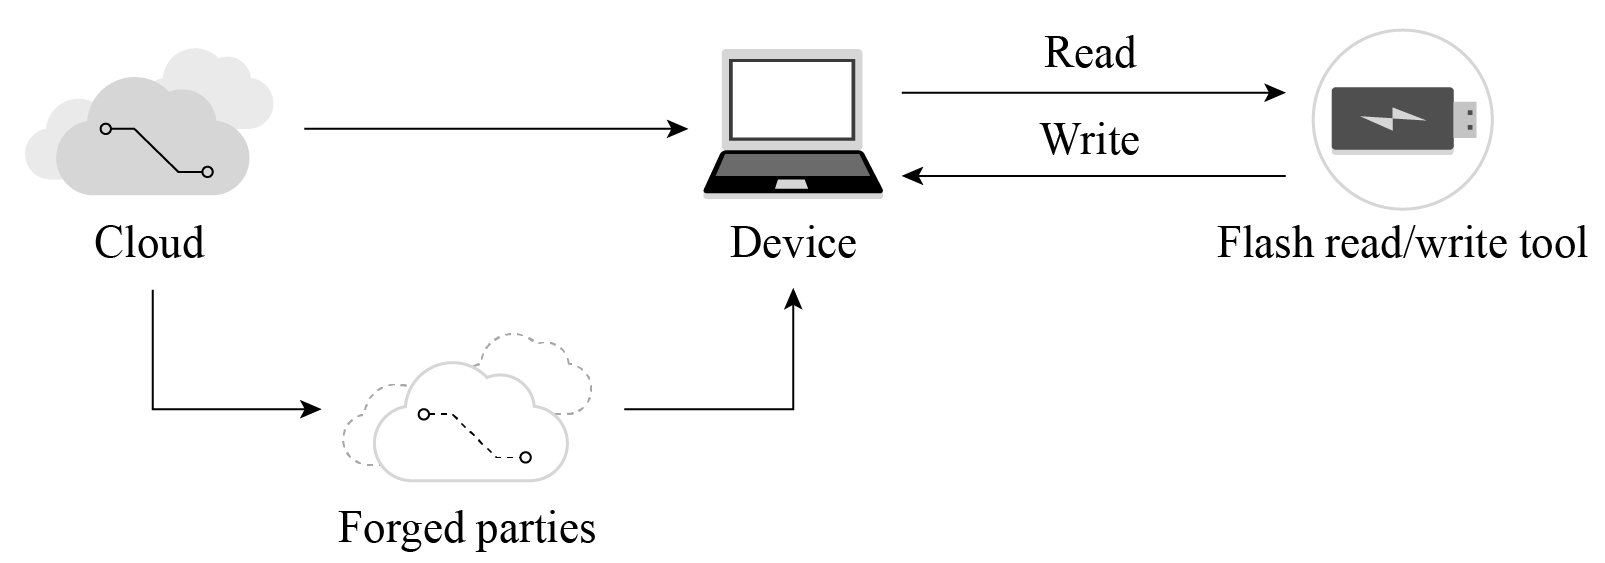
\includegraphics[width=0.7\textwidth]{D13Z/13-1}
    \caption{Security risks when exchanging data with cloud}
\end{figure}

As we can see, device data security cannot be guaranteed unless proper measures are taken. In real-world applications, threats to IoT devices are much more complex than those discussed above. As IoT devices often communicate with other devices and some may operate in unattended environments, it becomes easier for malicious actors to obtain, analyse, or tamper with the device's data. Therefore, ensuring data security has become a more urgent requirement.

\subsection{Basic Requirements for IoT Device Data Security}
Protecting the data security of IoT devices needs to be discussed from two aspects: data storage and data transmission. They respectively propose requirements for the protection of data integrity, confidentiality, and legality. The basic components of data security are shown in Figure 13.2.

\begin{figure}[!h]
    \centering
    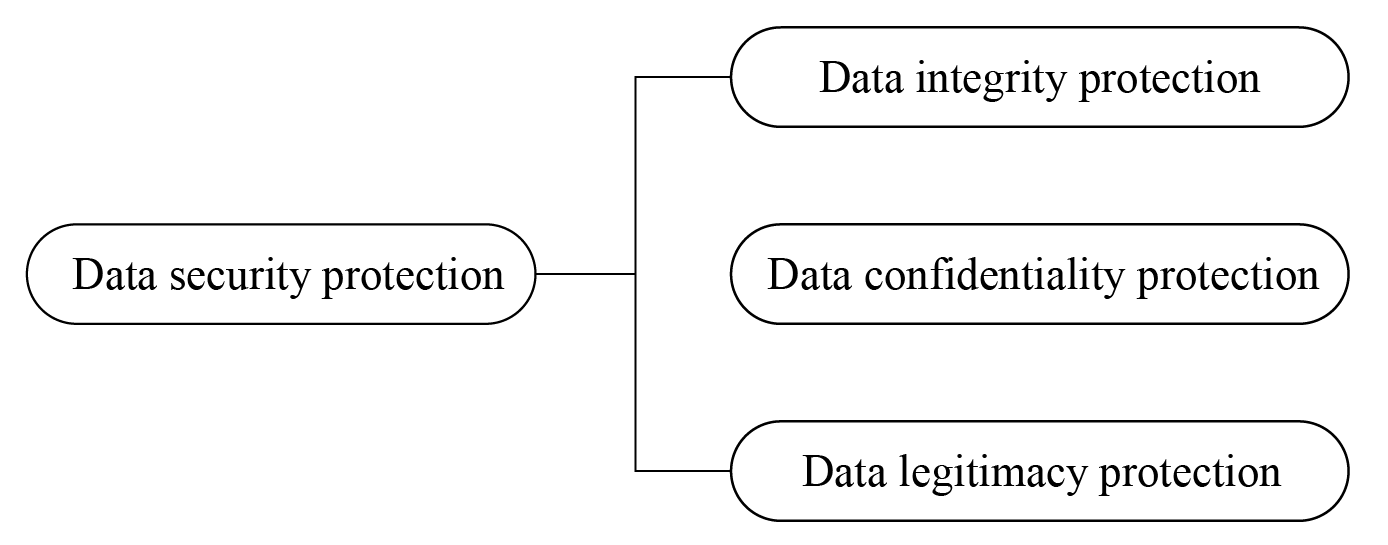
\includegraphics[width=0.55\textwidth]{D13Z/13-2}
    \caption{Basic components of data security}
\end{figure}

The requirements for data transmission security mainly include the following three aspects:

\begin{itemize}[noitemsep]
    \item Integrity: Data should not be tampered with or contain errors during transmission.
    \item Confidentiality: The data being transmitted is encrypted, and attackers cannot access the real content of the data.
    \item Legitimacy: The communicating peer device is a trusted target device.
\end{itemize}

The requirements for data storage security also include three aspects:

\begin{itemize}[noitemsep]
    \item Integrity: Data should not be tampered with or damaged during storage.
    \item Confidentiality: After the stored data is read, attackers cannot decipher the real content of the data.
    \item Legitimacy: The data being used is authenticated.
\end{itemize}

Of course, data storage security and transmission security are not completely independent. They complement each other and together constitute a unified framework for the security of IoT device data. After establishing the above framework, clarifying some concepts, and providing an understanding of the requirements for IoT device data security, this chapter will further explain how to protect IoT device data step by step.

\section{Data Integrity Protection}
\subsection{Introduction to Integrity Verification Method}
To verify data integrity, a block of data called checksum (also known as digest, fingerprint, hash value, or hash code) is usually used. The checksum is fixed-length check data generated by the corresponding integrity verification algorithm. The checksum essentially represents the uniqueness of the data block, just like a person’s fingerprint or ID number can uniquely represent this person. The integrity check algorithm is shown in Figure 13.3.

\begin{figure}[!h]
    \centering
    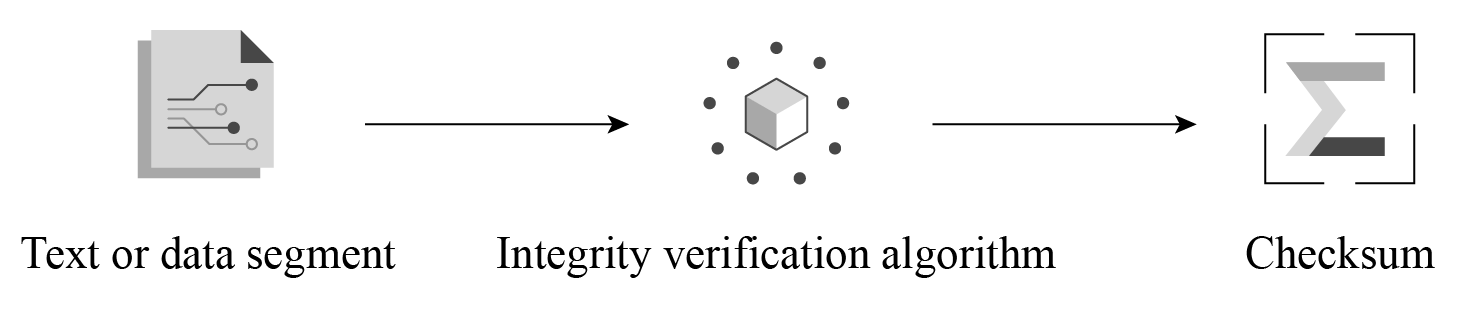
\includegraphics[width=0.7\textwidth]{D13Z/13-3}
    \caption{Integrity verification algorithm}
\end{figure}

The integrity verification algorithm has the following properties: 

\begin{term}{Collision resistance}
    Collision resistance means that within the data length specified by the algorithm, it is not feasible (or very difficult) to find two different data segments x and y that result in the same checksum. A collision happens when the size of data increases, some data is lost or damaged, but the correct checksum can be calculated.
\end{term}

\begin{term}{Raw data cannot be derived}
    In the case where the checksum is known, it is hard to figure out from the checksum what the raw data is.
\end{term}

A collision occurs when different pieces of data are input into the algorithm, resulting in the same checksum. Common integrity verification algorithms include CRC, MD5, SHA1, and SHA256. These algorithms generate checksums of varying lengths, which affects the likelihood of a collision. For example, the CRC32 checksum has a length of 32 bytes and can theoretically guarantee that data within 512 MB will not collide. However, the probability of data collision increases beyond this range.

A common way to perform data integrity verification is to append a checksum to the data to be verified. Figure 13.4 illustrates the basic principle of integrity verification, where a checksum is appended to the end of the data block. Upon receiving the data block, or prior to using the data, the receiver recalculates the checksum. If the calculated checksum matches the appended checksum, the data is deemed to be integral, otherwise the data is deemed to have been tampered with or to contain code errors.

\begin{figure}[!h]
    \centering
    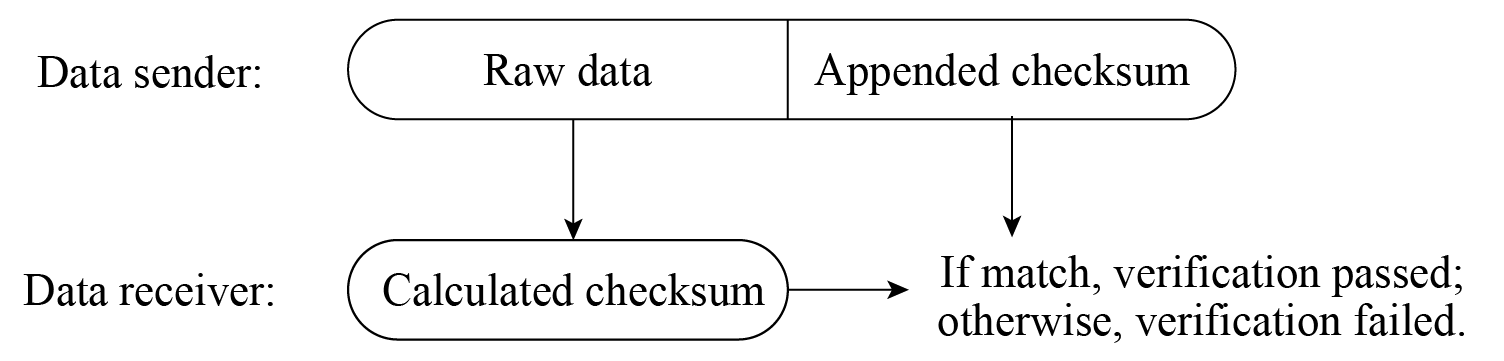
\includegraphics[width=0.6\textwidth]{D13Z/13-4}
    \caption{Basic principle of data integrity verification}
\end{figure}

\subsection{Integrity Verification of Firmware Data}
This section takes the integrity verification of firmware data during OTA upgrades as an example to introduce how data integrity verification is designed. Figure 13.5 shows that during firmware updates, integrity verification is performed before data transmission and updated firmware loading.

\begin{figure}[!h]
    \centering
    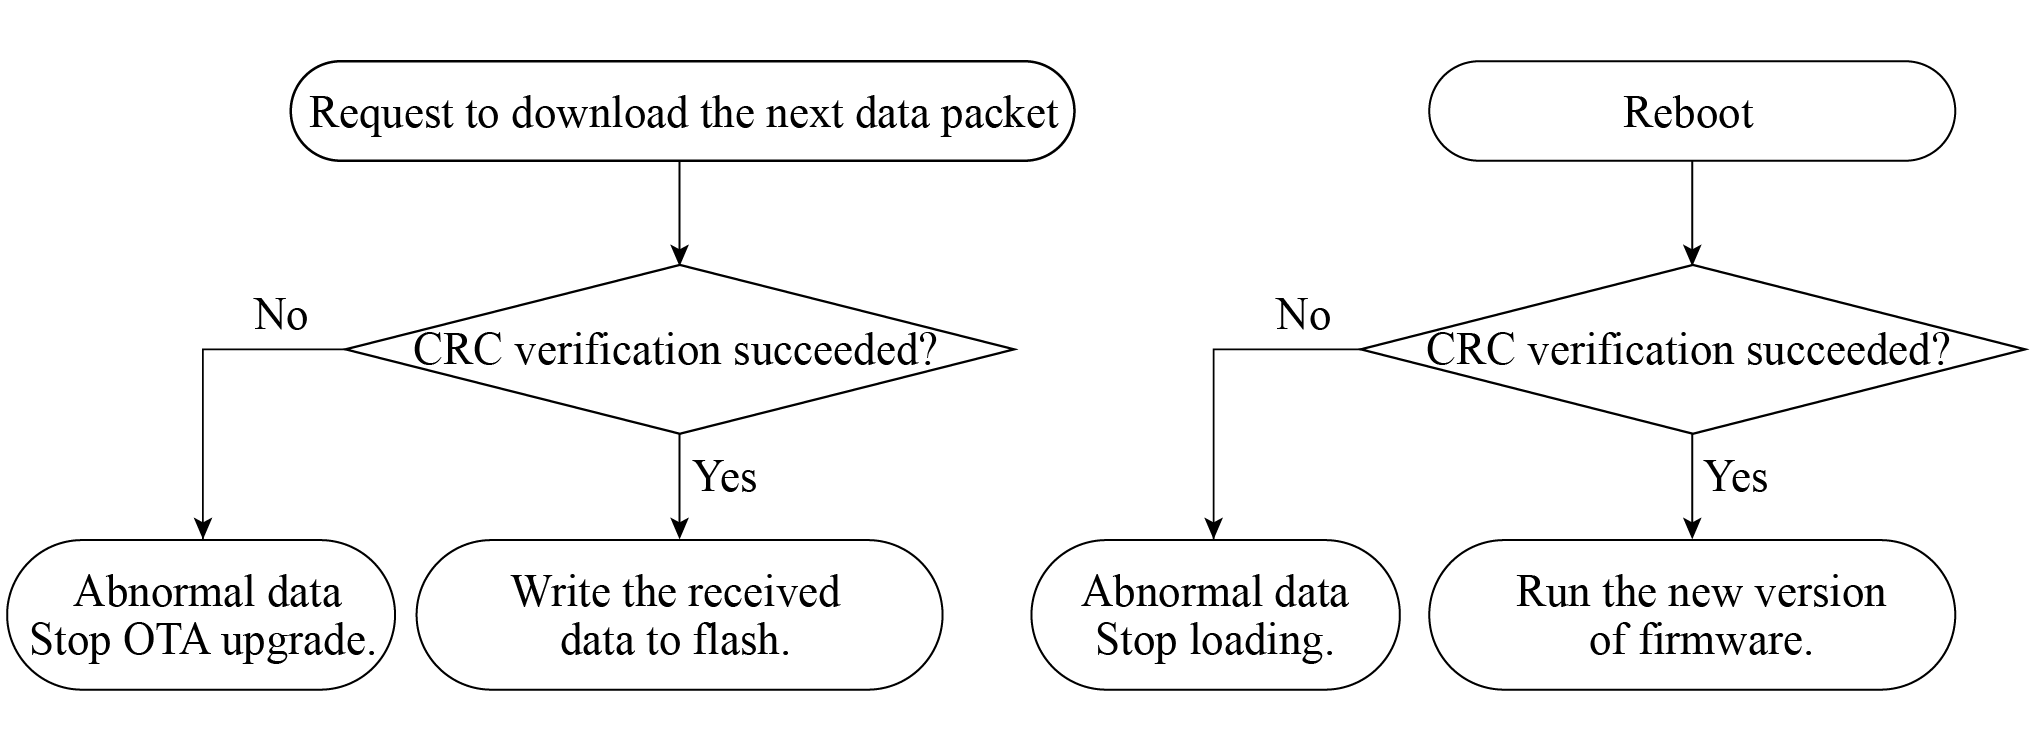
\includegraphics[width=0.9\textwidth]{D13Z/13-5}
    \caption{Integrity verification before data transmission and firmware loading}
\end{figure}

In the process of OTA upgrades, if HTTPS protocol is used to transmit data, the sender generates a CRC checksum for the data before transmission, and the receiver recalculates a CRC checksum from the received data, followed by verification similar to the process shown in Figure 13.4. It is worth noting that when using the HTTPS protocol to transmit data, there is no need to worry about CRC verification, as the HTTPS protocol automatically performs this verification internally.

In addition, when the device uses the firmware stored in flash, it also checks the integrity of the firmware. Every time the device is restarted to load the app firmware, it will perform integrity verification to ensure that the app firmware for loading is not damaged. This process occurs automatically and does not need manual intervention.

However, it is far from enough to rely only on integrity verification for ensuring data security. Since the mechanisms and implementations of the integrity verification algorithms are usually open-source, malicious attackers can use the same CRC verification algorithm to add a CRC checksum to a custom firmware and flash it into the device’s flash, thereby passing the CRC check. To prevent such attacks, it is necessary to identify the source of the data, which involves the data legitimacy protection scheme - Secure Boot, which will be covered in detail in Section 13.4.2.

\subsection{Example}
The Linux system integrates various tools for calculating checksums, such as \verb|sha256sum| and \verb|md5sum|. We can use these tools to calculate the checksum of specified files, and compare the changes of the checksums before and after modifying the file. 	Below commands use \verb|md5sum| to calculate the checksums of the \verb|hello.c| file before and after modification:

\begin{codebloc}
\begin{tabular}{d}
\$ \textbf{md5sum hello.c}

87cb921a75d4211a57ba747275e8bbe6 //Original MD5 checksum of hello.c

\$ \textbf{md5sum hello.c}

79c3416910f9ea0d65a72cb720368416 //New MD5 checksum after adding one line
\end{tabular}
\end{codebloc}

It can be seen that modifying just one line of code in the original file will result in greatly different MD5 checksums.

\section{Data Confidentiality Protection}
\subsection{Introduction to Data Encryption}
The purpose of data encryption is to prevent unauthorised entities from knowing the true meaning of the data, while enabling authorised users to interpret the data correctly. Now, suppose you wish to encrypt the data stored in the flash memory to prevent unauthorised access. First, you need to understand the key concepts as shown in Figure 13.6. The original data stored in flash is referred to as plaintext, while the encrypted data generated by the encryption algorithm is known as ciphertext. This ciphertext is incomprehensible to unauthorised entities. The encryption algorithm utilises a key, which is a string of numbers or characters. In the example presented in Figure 13.6, the encryption algorithm adds 1 to (the ASCII code of) each character in the original string and replaces all the characters. The key used by the encryption algorithm is an integer number 1. The decryption process is the reverse of the encryption process, where each character is changed by subtracting 1, thereby recovering the plaintext.

All data encryption algorithms are based on the principle of replacing one set of data with another. Figure 13.6 uses the simplest single-code replacement encryption algorithm. In real applications, encryption algorithms are much more complex, but the principle is the same.

\begin{figure}[!h]
    \centering
    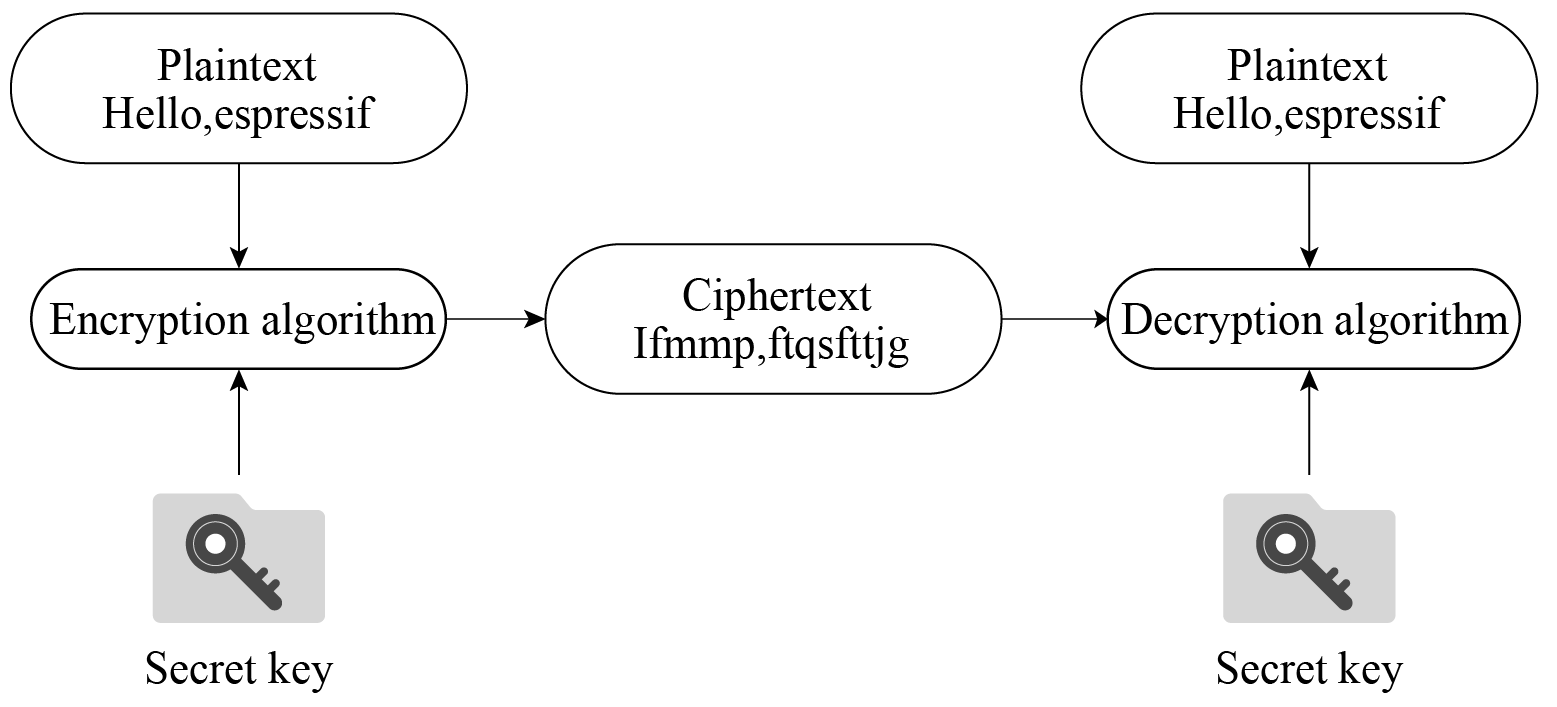
\includegraphics[width=0.7\textwidth]{D13Z/13-6}
    \caption{Basic principle of data encryption}
\end{figure}

Data encryption algorithms can generally be divided into two categories: symmetric encryption algorithms and asymmetric encryption algorithms.

\begin{term}{Symmetric encryption algorithms}
    As the name implies, symmetric encryption algorithms use the same key in both encryption and decryption process. Commonly used symmetric encryption algorithms include DES, 3DES, and AES. The encryption process shown in Figure 13.6 is the basic process of symmetric encryption. The key used for encryption and decryption is the same, that is, the integer number 1.
\end{term}

\begin{term}{Asymmetric encryption algorithms}
    The asymmetric encryption algorithms use two different keys: public key and private key, which are a pair of strings with a specific association. The content encrypted by the public key can only be decrypted by the paired private key. Similarly, the content encrypted by the private key can only be decrypted by the paired public key.
\end{term}

A prerequisite for symmetric encryption is that the encryptor and the decryptor must agree on a shared key, that is, they must know the content of the key beforehand. However, in some cases, the encryptor and decryptor have never met, nor exchanged data through any means other than the network. In such cases without pre-agreed keys, how can the encryptor and decryptor perform encryption or decryption? The answer is asymmetric encryption algorithm.

Figure 13.7 shows the basic process of using asymmetric encryption and symmetric encryption together to transmit encrypted data, where asymmetric encryption is used to exchange the key used for encryption, and after getting the symmetric key, the client and server use the less resource-intensive symmetric encryption algorithm to protect the confidentiality of transmitted data.

\begin{figure}[!h]
    \centering
    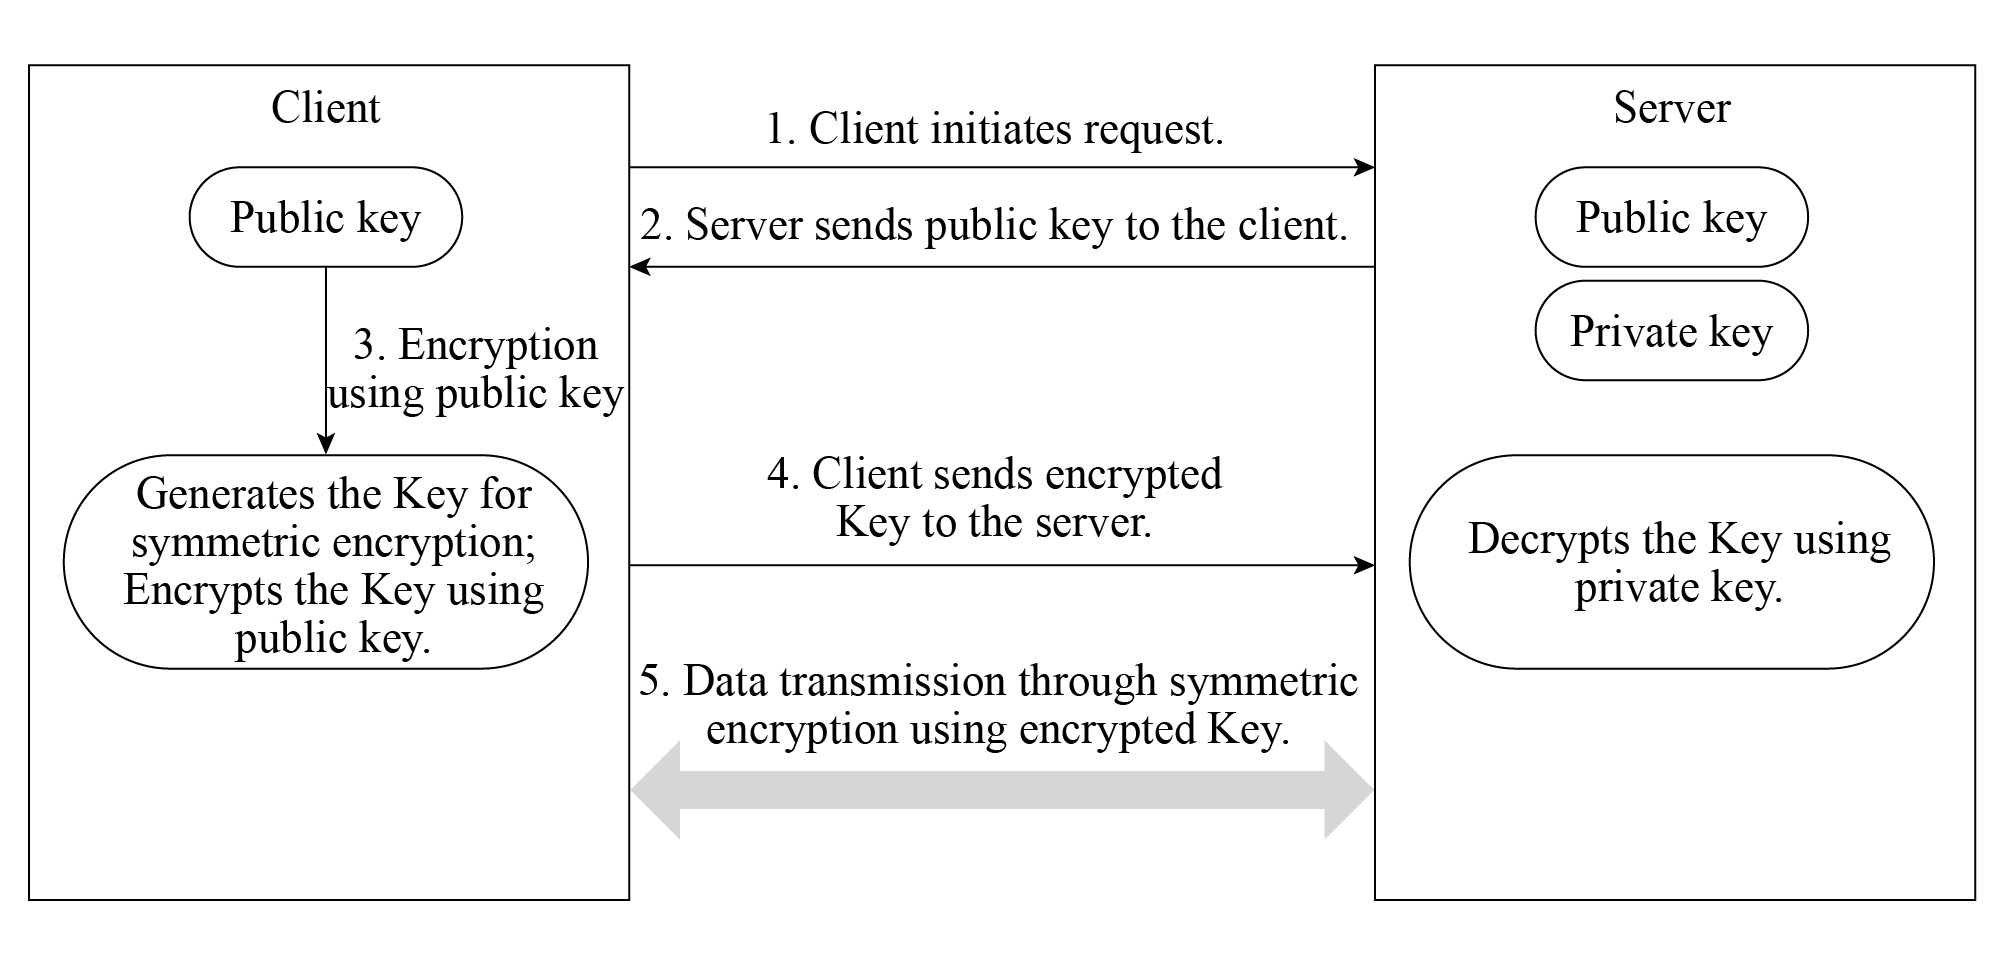
\includegraphics[width=0.7\textwidth]{D13Z/13-7}
    \caption{Combining asymmetric and symmetric encryption to transmit data}
\end{figure}

The commonly-used asymmetric encryption algorithm is RSA algorithm.

Technical details about encryption algorithms will not be provided in this book. After gaining a foundational understanding of data encryption, we can proceed to a new journey.

\subsection{Introduction to Flash Encryption Scheme}
Flash encryption is used to enhance the protection of data confidentiality so as to ensure data security. Once this feature is enabled, physical readout of flash will not be sufficient to recover flash contents. As explained above, data confidentiality needs to be protected during both transmission and storage stages. Flash encryption can be used to encrypt data stored in flash, while other encryption scheme is needed for data transmission, for example HTTPS transmission protocol.

\subsubsection{1. Relevant storage areas}
Both eFuse and flash are storage media relevant to the flash encryption scheme, but have different properties and usages, as shown in Table 13.1.

\begin{table}[h!]
    \renewcommand{\arraystretch}{1.4}
    \caption{Contents and properties of eFuse and flash}
    \begin{tabular}{|>{\Centering}m{5em}|>{\RaggedRight}m{15em}|>{\RaggedRight}m{18em}|}
        \hline
        \rowcolor{LightBlue} \textbf{Storage medium}&\multicolumn{1}{c|}{\textbf{Contents}}&\multicolumn{1}{c|}{\textbf{Properties}}\\
        \hline
        Flash&\verb|Bootloader.bin|, \verb|app.bin|,\newline\verb|nvs| data, and partition tables&Flash memory can be erased and reprogrammed repeatedly.\\
        \hline
        eFuse&System parameters such as chip version and MAC, and keys and control bits relevant to system functions&Once an eFuse bit is programmed to 1, it can never be reverted to 0. In particular, for some eFuse blocks, if they are set to be read-protected, the data in these blocks can only be read by hardware cryptography modules.\\
        \hline
    \end{tabular}
\end{table}

The types of data that are stored in the flash and encrypted by flash encryption include firmware bootloader, app firmware, partition table, and any partition marked with the \verb|encrypted| flag in the partition table.

Taking the following partition table as an illustration, enabling flash encryption will result in the encryption of specific partitions, namely the bootloader partition, factory partition, storage partition, and nvs\_key partition. Notably, partitions used to store firmware, such as the bootloader partition and factory partition, are encrypted by default, so there is no need to add \verb|encrypted| flag to them.

\begin{codebloc}
\begin{tabular}{d}
\vspace{2pt}
\fontsize{9.5pt}{10pt}\selectfont
\begin{verbatim}
1.  # Name,   Type, SubType, Offset,  Size, Flags
2.  nvs,        data, nvs,      ,  0x6000,
3.  # Extra partition to demonstrate reading/writing of encrypted flash
4.  storage,    data, 0xff,     ,  0x1000, encrypted
5.  factory,    app,  factory,  , 1M,
6.  # nvs_key partition contains the key that encrypts the NVS partition named nvs.
7.  The nvs_key partition needs to be encrypted.
\end{verbatim}
\verb|8.  nvs_key,    data, nvs_keys, , 0x1000, encrypted,|
\end{tabular}
\end{codebloc}

Flash encryption is used to encrypt data stored in flash. Some eFuses are used during flash encryption. The list of utilised eFuses and their descriptions are given in Table 13.2.

\begin{table}[h!]
    \renewcommand{\arraystretch}{1.3}
    \caption{eFuses used in flash encryption}
    \begin{tabular}{|m{11em}|>{\RaggedRight}m{23em}|>{\Centering}m{4em}|}
        \hline
        \rowcolor{LightBlue} \multicolumn{1}{|c|}{\textbf{eFuses}}&\multicolumn{1}{c|}{\textbf{Description}}&\textbf{Length (bit)}\\
        \hline
        \texttt{BLOCK\_KEY\textit{N}}&Used to store flash encryption/decryption key.\newline \textit{N} ranges from 0 to 4.&256\\
        \hline
        \verb|DIS_DOWNLOAD_|\newline \verb|MANUAL_ENCRYPT|&If set, disables flash encryption download function in download boot mode.&1\\
        \hline
        \verb|SPI_BOOT_CRYPT_CNT|&Enables encryption and decryption.\newline Feature is enabled if one or three bits are set in the eFuse, disabled otherwise.&3\\
        \hline
    \end{tabular}
\end{table}

The tool \verb|espefuse.py| can be used to check the current eFuse status on ESP32-C3. For example, run the following command to check the current eFuse value:

\begin{codebloc}
\begin{tabular}{d}
\$ \textbf{espefuse.py --port PORT summary}   //replace "PORT" with your port name
\end{tabular}
\end{codebloc}

If \verb|FLASH_CRYPT_CNT| is 0, as shown in the log below, it means flash encryption is not enabled.

\begin{codebloc}
\begin{tabular}{d}
\vspace{2pt}
\begin{verbatim}
espefuse.py v2.6-beta1
Connecting........_____.
EFUSE_NAME          Description = [Meaningful Value] [Readable/Writeable] (Hex 
Value)
----------------------------------------------------------------------------
Security fuses:
FLASH_CRYPT_CNT        Flash encryption mode counter            = 0 R/W (0x0)
FLASH_CRYPT_CONFIG     Flash encryption config (key tweak bits) = 0 R/W (0x0)
CONSOLE_DEBUG_DISABLE  Disable ROM BASIC interpreter fallback   = 1 R/W (0x1)

Identity fuses:
MAC                   MAC Address                                       
  = 30:ae:a4:c3:86:94 (CRC 99 OK) R/W 
\end{verbatim}
\verb|...|
\end{tabular}
\end{codebloc}

\subsubsection{2. Flash encryption algorithm}
The symmetric encryption algorithm used by flash encryption is AES-XTS, which is a tweakable block cipher. During encryption, the algorithm encrypts plaintext data in blocks, and dynamically adjusts the key according to the offset address of the plaintext data. The basic principle of AES-XTS-128 block encryption is shown in Figure 13.8, where the plaintext data of 64 Bytes are divided into four blocks, and the encryption keys (key1 $\sim$ key4) are derived from \verb|base_key|. Combining the four encrypted blocks will get the 64 B encrypted data.

\begin{figure}[!h]
    \centering
    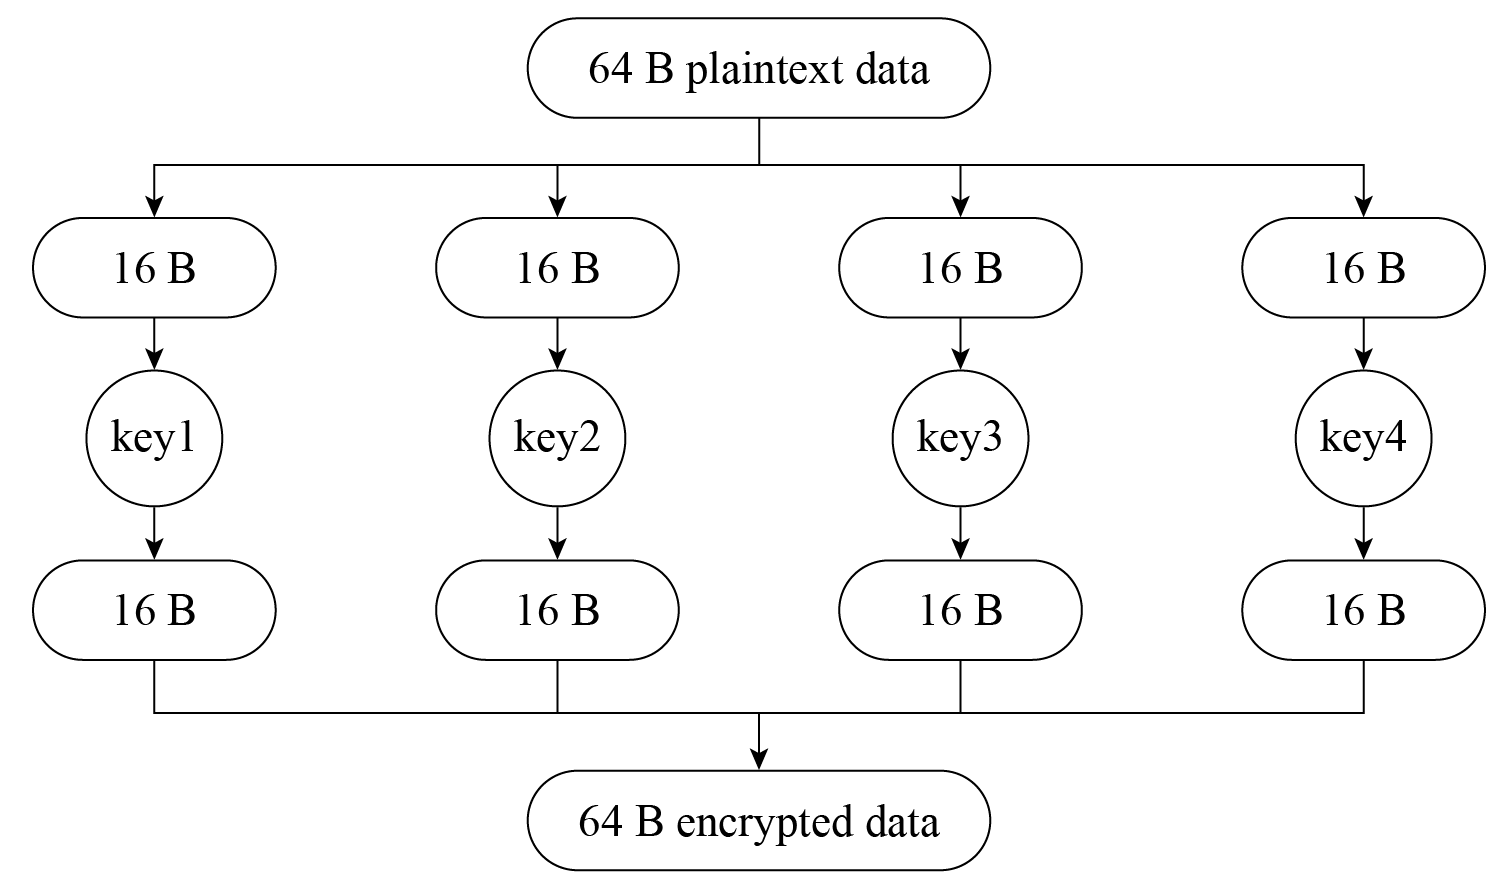
\includegraphics[width=0.62\textwidth]{D13Z/13-8}
    \caption{Basic principle of AES-XTS-128 block encryption}
\end{figure}

The benefits of AES-XTS, which first dynamically adjusts the encryption key and then encrypts data, are: 

\begin{itemize}
    \item Encrypting the same data block results in different ciphertext, which makes the encrypted data more difficult to be analysed and cracked, thus increasing data confidentiality. 
    \item Different data blocks can be encrypted and decrypted independently. Even if one data block is damaged, it will not affect the decryption of other data blocks. Encryption/decryption between data blocks is independent.
\end{itemize}

\subsection{Flash Encryption Key Storage}
The flash encryption key is stored in \verb|BLOCK_KEY|. There are two methods to write the key into eFuse: 

\begin{term}{Manual method}
    Use \verb|espsecure.py| to manually generate a key and write it into eFuse. This method can only be used before enabling flash encryption for the first time.
\end{term}

\begin{term}{Automatic method}
    After flash encryption is enabled in \verb|menuconfig|, the device will automatically generate a key in the bootloader when it starts up for the first time, and automatically save the key in eFuse.
\end{term}

To manually write the flash encryption key into eFuse, first run the following command to generate the key:

\begin{codebloc}
\begin{tabular}{d}
\$ \textbf{espsecure.py generate\_flash\_encryption\_key my\_flash\_encryption\_key.bin}
\end{tabular}
\end{codebloc}

Then, run the following command to write the key into eFuse:

\begin{codebloc}
\begin{tabular}{d}
\fontsize{9.5pt}{10pt}\selectfont
\$ \textbf{espefuse.py --port PORT burn\_key BLOCK my\_flash\_encryption\_key.bin XTS\_AES\_128\_KEY}
\end{tabular}
\end{codebloc}

\note{Since writing eFuse is irreversible, manual writing of the key into eFuse can only be performed once.}

Flash encryption can be enabled through \verb|menuconfig → Security features → |\\ \verb|Enable flash encryption on boot|. If flash encryption is enabled in building stage and the key has not been manually written into eFuse in advance, then after the firmware is flashed, the device will enable flash encryption, automatically generate a key, and write it into eFuse.

The main difference between the manual method and automatic method is that with the manual method, you can know the content of the key and use a script tool to encrypt the data before flashing it into the device. With the automatic method, if the read protection of \verb|BLOCK_KEY| is enabled in the eFuse (which is enabled by default), the key is generated inside the device and stored directly in the read-protected eFuse, making it impossible for external developers to obtain the key or manually encrypt/decrypt the data.

In manual mode, use the following command to encrypt the app firmware, and flash it to the device:

\begin{codebloc}
\begin{tabular}{d}
\$ \textbf{espsecure.py encrypt\_flash\_data --aes\_xts --keyfile /path/to/key.bin --address 0x10000 --output my-app-ciphertext.bin build/my-app}
\end{tabular}
\end{codebloc}

It is important to note that when using the aforementioned command for data encryption, you must specify the storage address of the data in the partition table. In the command provided, the data being encrypted is \verb|my-app|, with its address set to 0x10000. As emphasised in Section 13.3.2, flash encryption relies on the tweakable block cipher AES-XTS, and therefore, the accurate data address must be specified. Failure to specify or incorrectly specifying the address will result in device failure after flashing the encrypted firmware.

Furthermore, it is worth mentioning that if the encryption key is known, the script tool \verb|espsecure.py| can also be used to decrypt the data. Running the command \verb|espsecure|\\ \verb|.py-h| will provide helpful information regarding the usage of the script tool.

During the mass production of devices, it is highly recommended to utilise the automatic method for key writing. This ensures that each device is assigned a unique key that remains inaccessible from external sources, thus maximising the overall security of the device.

\subsection{Working Mode of Flash Encryption}
Flash encryption has two working modes: 

\begin{term}{Development mode}
    As the name suggests, development mode is used during the development stage where there is a frequent need to program different plaintext flash images and test the flash encryption process. This requires that new plaintext images can be loaded as many times as needed. In development mode, flash encryption can be disabled and new firmware can be flashed using commands, which will be explained in Section 13.3.7.
\end{term}

\begin{term}{Release mode}
    Release mode is recommended for mass production. In release mode, serial port cannot perform flash encryption operations, which can be ensured by enabling flash encryption feature. In this mode, flash encryption cannot be disabled once enabled, and new firmware cannot be downloaded over serial port but only be downloaded using the over-the-air (OTA) scheme.
\end{term}

The working mode of flash encryption can be selected through \verb|menuconfig → security|\\ \verb|features → Enable flash encryption on boot → Enable usage mode|. Figure 13.9 shows that development mode is enabled for flash encryption.

\begin{figure}[!h]
    \centering
    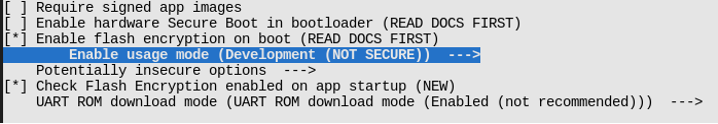
\includegraphics[width=0.8\textwidth]{D13Z/13-9}
    \caption{Development mode enabled for flash encryption}
\end{figure}

Note that in development mode, flash encryption can be disabled with \verb|espefuse.py|\\ \verb|--port PORT burn_efuse SPI_BOOT_CRYPT_CNT|. After disabling encryption scheme, deselect the option in \verb|menuconfig|, then run \verb|idf.py flash| to flash new firmware. The number of times to disable flash encryption is limited by the length of the \verb|SPI_BOOT_CRYPT|\\ \verb|_CNT| flag in eFuse. If the flag contains an odd number of “1”s, it means that flash encryption is enabled; if it contains an even number of “1”s, it means that flash encryption is disabled. If the length of the flag bit is 3 bits, it means flash encryption can only be disabled once.

\note{Visit \url{https://docs.espressif.com/projects/esptool/en/latest/esp32/espsecure/index.html} for more information about \texttt{espefuse.py}.}

Enabling flash encryption may increase the size of bootloader. Options to work around this are: 

\begin{enumerate}[label=(\arabic*)]
    \item Set partition table offset through \verb|menucofig → Partition Table → Offset|\\ \verb|of partition table|. For example, changing the offset from 0x8000 to 0xa000 will increase the space by 8 KB.
    
    Note that after changing the partition offset of the bootloader, you need to check whether the area allocation in the partition table needs to be updated.

    \item Reduce bootloader log level through \verb|menuconfig → Bootloader log verbo-|\\ \verb|sity|. Changing log level from Info to Warning can reduce log size, thus reducing the bootloader size.
\end{enumerate}

\subsection{Flash Encryption Process}
After flashing the plaintext firmware to the device with flash encryption enabled for the first time, and subsequently starting the device, the flash encryption feature will be automatically enabled. The following outlines the basic workflow for the initial automatic enabling of flash encryption:

\begin{enumerate}[label=(\arabic*)]
    \item Firmware bootloader reads the \verb|SPI_BOOT_CRYPT_CNT| eFuse value. If flash encryption is not enabled, the bootloader will enable flash encryption. By default, the value is 0, meaning flash encryption is not enabled yet.
    \item Bootloader checks if \verb|BLOCK_KEY| stores the flash encryption key. If the key is not pre-flashed (see Section 13.3.3), it will be generated automatically and written to \verb|BLOCK_KEY|. The write and read protection bits for \verb|BLOCK_KEY| will be set, so that software cannot access the key.
    \item Flash encryption block encrypts the flash contents - the firmware bootloader, applications and partitions marked as \verb|encrypted|.
    \item Firmware bootloader sets the first available bit in \verb|SPI_BOOT_CRYPT_CNT| to 1 to mark the flash contents as encrypted.
    \item In Development mode, \verb|SPI_BOOT_CRYPT_CNT| and \verb|DIS_DOWNLOAD_MANUAL_ENC|\\ \verb|RYPT| are not write-protected. The firmware bootloader allows to disable flash encryption and re-flash encrypted binaries.
    \item In Release mode, \verb|SPI_BOOT_CRYPT_CNT| and \verb|DIS_DOWNLOAD_MANUAL_ENCRYPT| are write-protected. Flash encryption is enabled permanently and re-flashing firmware is forbidden.
    \item The device is rebooted to start executing the encrypted bootloader and app firmware.
\end{enumerate}

\note{By default, when flash encryption is enabled, some flag bits of eFuse will be set, thus disabling some system functions, such as JTAG. Keeping these system functions may bring security risks. During test phase, if you need to keep these flags, please refer to the instructions related to flash encryption in the ESP-IDF Programming Guide.}

With flash encryption enabled, when the device loads and runs encrypted bootloader and app firmware, it first automatically decrypts the data through the hardware module, and then loads the decrypted data into its iRAM and cache. Furthermore, certain APIs are designed to seamlessly handle the encryption and decryption of data when performing read and write operations within encrypted partitions in the flash memory. The APIs responsible for automatic decryption of data include \verb|esp_partition_read()|, \verb|esp_flash_read_|\\ \verb|encrypted()|, and \verb|bootloader_flash_read()|; the APIs responsible for automatic encryption of data include \verb|esp_partition_write()|, \verb|esp_flash_write_encrypted()|, and \verb|bootloader_flash_write()|.

Particularly, with flash encryption enabled, during OTA upgrades, the device receives plaintext data, and then calls \verb|esp_partition_write()| to automatically encrypt the data before writing it into the flash memory.

\note{For mass-produced devices, OTA upgrade function can be used to update app firmware remotely, but not the bootloader. Therefore, it is crucial to carefully configure the bootloader settings, including parameters like the log level, before enabling flash encryption.}

\subsection{Introduction to NVS Encryption}
The flash encryption scheme does not directly protect the data stored in the NVS partition. To protect the confidentiality of the data stored in NVS partition, NVS encryption scheme should be used. NVS encryption can be enabled through \verb|menuconfig → Component |\\ \verb|config → NVS → Enable NVS encryption| or by calling \verb|nvs_flash_secure_|\\ \verb|init()|.

The basic principle of the NVS encryption scheme is to define a partition in the partition table with a size of no less than 4 KB and the subtype of \verb|nvs_key|. After enabling the NVS encryption scheme, the NVS partition will be encrypted using the key in the \verb|nvs_key| partition. A typical partition table that supports NVS encryption is shown below:

\begin{codebloc}
\begin{tabular}{d}
\vspace{2pt}
\begin{verbatim}
1.  # Name,     Type,   SubType,    Offset, Size,   Flags
2.  nvs,        data,   nvs,        ,       0x6000,
3.  phy_init,   data,   phy,        ,       0x1000,
4.  factory,    app,    factory,    ,       1M,
\end{verbatim}
\verb|5.  nvs_key,    data,   nvs_keys,   ,       0x1000, encrypted,|
\end{tabular}
\end{codebloc}

NVS encryption scheme is similar to the flash encryption scheme in many ways, such as:

\begin{itemize}[leftmargin=1em]
    \item The encryption algorithm used by the NVS encryption scheme is the symmetric encryption algorithm AES-XTS. As mentioned earlier, symmetric encryption algorithm requires its key to be kept secret to ensure that the encrypted data cannot be analysed and cracked. The key of the NVS encryption scheme cannot be plaintext, so this scheme is often used together with the flash encryption scheme, where flash encryption is responsible for protecting the confidentiality of the \verb|nvs_key|, while NVS encryption uses \verb|nvs_key| to protect the confidentiality of the NVS partition.
    \item There are two methods for storing the NVS encryption key: one is the manual method, that is, manually generate a key and write the key to the designated partition; the other is the automatic method, that is, when the NVS encryption scheme is first enabled and the \verb|nvs_key| partition is empty, the device automatically calls the \verb|nvs_flash_generate_|\\ \verb|keys()| function to generate the key, and then writes the key to the \verb|nvs_key| partition, and subsequently uses the key to complete NVS encryption/decryption.

    The steps to manually store the NVS encryption key are as follows:

    First, generate a file containing the key by running the following command:
    
    \begin{codebloc}
    \begin{tabular}{a}
    \$ \textbf{espsecure.py generate\_flash\_encryption\_key my\_nvs\_encryption\_key.bin}
    \end{tabular}
    \end{codebloc}
    
    Then, compile and burn the partition table with the following command:
    
    \begin{codebloc}
    \begin{tabular}{a}
    \$ \textbf{idf.py -p (PORT) partition\_table-flash}
    \end{tabular}
    \end{codebloc}
    
    Finally, burn the key to the specified partition with the following command:
    
    \begin{codebloc}
    \begin{tabular}{a}
    \$ \textbf{parttool.py -p (PORT) --partition-table-offset "nvs\_key partition offset" write\_partition --partition-name="name of nvs\_key partition" --input "nvs\_key partition"}
    \end{tabular}
    \end{codebloc}

    \item After enabling NVS encryption, APIs starting with \verb|nvs_get| or \verb|nvs_set| automatically perform data encryption/decryption when reading/writing data in the NVS partition.
\end{itemize}

Please note that when flash encryption is enabled, it is highly recommended to also enable NVS encryption (which is enabled by default). This is important because the Wi-Fi driver stores sensitive data, such as SSID and password, in the default NVS partition. The NVS encryption scheme allows for the use of different keys (\verb|nvs_key|) in different NVS partitions. When initialising a specific NVS partition, you only need to specify the corresponding \verb|nvs_key|. 

\note{Visit \url{https://bookc3.espressif.com/nvs} for further information about NVS encryption.}

\subsection{Examples of Flash Encryption and NVS Encryption}
In the \href{https://github.com/espressif/esp-idf/tree/master/examples/security/flash_encryption}{\texttt{esp-idf/examples/security/flash\_encryption}} directory, we’ve uploaded an example of flash encryption and NVS encryption. By running this example, you can observe the logs that demonstrate the results of flash encryption and NVS encryption.

As mentioned earlier, when flash encryption is enabled in development mode, the firmware can be flashed repeatedly. To flash the firmware into the device, we have used the following three commands:

\textbf{Command 1:}

\begin{codebloc}
\begin{tabular}{d}
\$ \textbf{idf.py -p PORT flash monitor}
\end{tabular}
\end{codebloc}

\textbf{Command 2:}

\begin{codebloc}
\begin{tabular}{d}
\$ \textbf{idf.py -p PORT encrypted-flash monitor}
\end{tabular}
\end{codebloc}

\textbf{Command 3:}

\begin{codebloc}
\begin{tabular}{d}
\$ \textbf{idf.py -p PORT encrypted-app-flash monitor}
\end{tabular}
\end{codebloc}

The results of running the above three commands are:

\begin{itemize}[leftmargin=1.5em,noitemsep]
    \item Command 1: the data stored in flash remains plaintext, resulting in a loading error;
    \item Command 2: only the encrypted bootloader, app firmware, and partition table are flashed, and can be loaded and run on the device without any issues;
    \item Command 3: only the encrypted app firmware is flashed; if the bootloader is also encrypted, the firmware can be loaded and run on the device.
\end{itemize}

The above three commands actually call \verb|esptool.py| internally. The corresponding settings of \verb|esptool.py| are:

\begin{codebloc}
\begin{tabular}{d}
\$ \textbf{esptool.py --chip esp32c3 -p /dev/ttyUSB0 -b 460800 --before=default\_reset --after= no\_reset write\_flash --flash\_mode dio --flash\_freq 40m --flash\_size 2MB 0x1000 bootloader/bootloader 0x20000 flash\_encryption.bin 0xa000 partition\_table/partition-table.bin}

\vspace{12pt}
\$ \textbf{esptool.py --chip esp32c3 -p /dev/ttyUSB0 -b 460800 --before=default\_reset --after= no\_reset write\_flash --flash\_mode dio --flash\_freq 40m --flash\_size 2MB --encrypt 0x1000 bootloader/bootloader 0x20000 flash\_encryption.bin 0xa000 partition\_table/partition-table.bin}

\vspace{12pt}
\$ \textbf{esptool.py --chip esp32c3 -p /dev/ttyUSB0 -b 460800 --before=default\_reset --after= no\_reset write\_flash --flash\_mode dio --flash\_freq 40m --flash\_size 2MB --encrypt 0x20000 flash\_encryption.bin}
\end{tabular}
\end{codebloc}

By examining the settings of the commands, we can conclude that when using \verb|esptool.py| for flashing, adding the option \verb|--encrypt| will enable automatic flash encryption and write the encrypted data into flash.

Below are several typical failure cases when enabling flash encryption:

\begin{itemize}[leftmargin=1em]
    \item If the \textbf{bootloader} is plaintext, the following failure may occur when starting the device:

\begin{codebloc}
\begin{tabular}{a}
\begin{verbatim}
rst:0x3 (SW_RESET),boot:0x13 (SPI_FAST_FLASH_BOOT)
invalid header: 0xb414f76b
invalid header: 0xb414f76b
invalid header: 0xb414f76b
invalid header: 0xb414f76b
invalid header: 0xb414f76b
invalid header: 0xb414f76b
\end{verbatim}
\vspace{-6pt}
\verb|invalid header: 0xb414f76b|
\end{tabular}
\end{codebloc}

    \item If the \textbf{partition} is plaintext, the following failure may occur when starting the device:

\begin{codebloc}
\begin{tabular}{a}
\begin{verbatim}
rst:0x3 (SW_RESET),boot:0x13 (SPI_FAST_FLASH_BOOT)
configsip: 0, SPIWP:0xee
clk_drv:0x00,q_drv:0x00,d_drv:0x00,cs0_drv:0x00,hd_drv:0x00,wp_drv:0x00
mode:DIO, clock div:2
load:0x3fff0018,len:4
load:0x3fff001c,len:10464
ho 0 tail 12 room 4
load:0x40078000,len:19168
load:0x40080400,len:6664
entry 0x40080764
\end{verbatim}
\vspace{-6pt}
\verb|I (60) boot: ESP-IDF v4.0-dev-763-g2c55fae6c-dirty 2nd stage bootloader|
\end{tabular}
\end{codebloc}

\begin{codebloc}
\begin{tabular}{a}
\begin{verbatim}
I (60) boot: compile time 19:15:54
I (62) boot: Enabling RNG early entropy source...
I (67) boot: SPI Speed       : 40MHz
I (72) boot: SPI Mode        : DIO
I (76) boot: SPI Flash Size : 4MB
E (80) flash_parts: partition 0 invalid magic number 0x94f6
E (86) boot: Failed to verify partition table
\end{verbatim}
\vspace{-6pt}
\verb|E (91) boot: load partition table error!|
\end{tabular}
\end{codebloc}

    \item If the \textbf{app firmware} is plaintext, the following failure may occur when starting the device:

\begin{codebloc}
\begin{tabular}{a}
\begin{verbatim}
rst:0x3 (SW_RESET),boot:0x13 (SPI_FAST_FLASH_BOOT)
configsip: 0, SPIWP:0xee
clk_drv:0x00,q_drv:0x00,d_drv:0x00,cs0_drv:0x00,hd_drv:0x00,wp_drv:0x00
mode:DIO, clock div:2
load:0x3fff0018,len:4
load:0x3fff001c,len:8452
load:0x40078000,len:13616
load:0x40080400,len:6664
entry 0x40080764
I (56) boot: ESP-IDF v4.0-dev-850-gc4447462d-dirty 2nd stage bootloader
I (56) boot: compile time 15:37:14
I (58) boot: Enabling RNG early entropy source...
I (64) boot: SPI Speed      	: 40MHz
I (68) boot: SPI Mode       	: DIO
I (72) boot: SPI Flash Size	: 4MB
I (76) boot: Partition Table:
I (79) boot: ## Label           Usage          Type ST Offset   Length
I (87) boot:  0 nvs             Wi-Fi data      01 02 0000a000 00006000
I (94) boot:  1 phy_init        RF data         01 01 00010000 00001000
I (102) boot:  2 factory        factory app     00 00 00020000 00100000
I (109) boot: End of partition table
E (113) esp_image: image at 0x20000 has invalid magic byte
W (120) esp_image: image at 0x20000 has invalid SPI mode 108
W (126) esp_image: image at 0x20000 has invalid SPI size 11
E (132) boot: Factory app partition is not bootable
\end{verbatim}
\vspace{-6pt}
\verb|E (138) boot: No bootable app partitions in the partition table|
\end{tabular}
\end{codebloc}

\end{itemize}

\section{Data Legitimacy Protection}
\subsection{Introduction to Digital Signature}
You may have signed your name on an application for admission, legal documents, or credit card receipts, indicating that you agree with the content of these documents. In the field of data security, the device needs to identify the sender or the producer of the data to indicate that the data is not forged, has been authorised, is legitimate, and can be used safely. Digital signature is a technical solution for verifying data legitimacy.

Digital signature has two properties: \textbf{unforgeability}, that is, only legitimate data senders can sign data, and other signatures are invalid; \textbf{verifiability}, that is, data users must be able to verify the validity of the signature.

Common digital signature algorithms include \textbf{RSA} and \textbf{DSA}. The basic process of digital signature verification is:

\begin{enumerate}[label=(\arabic*)]
    \item The data sender generates a private key, which is used to generate a public key, thus getting a private-public key pair. Note that only the private key can generate a matching public key.
    \item The data sender saves the public key to the storage system of the data user.
    \item The data sender signs the data with the private key and sends the signed data and signature to the data user.
    \item After receiving the data, the data user uses the public key stored in step (2) to verify the signature sent in step (3). If the signature is correct, the data is considered to be from a legitimate data sender; otherwise, the data is considered unauthorised and will not be used.
\end{enumerate}

The basic principle of using digital signature to verify data legitimacy is shown in Figure 13.10.

\begin{figure}[!h]
    \centering
    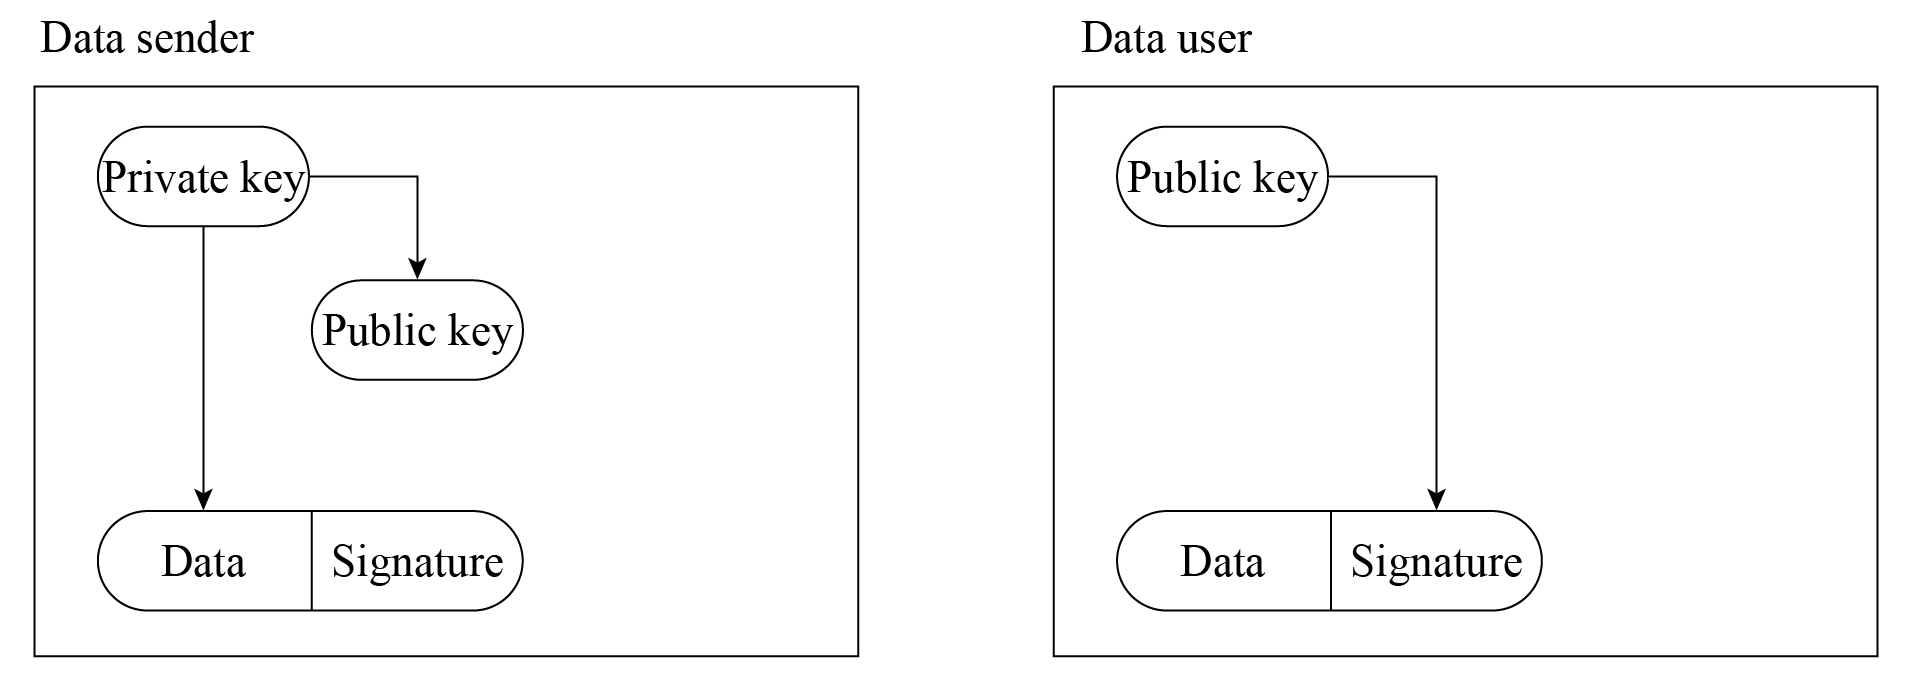
\includegraphics[width=0.8\textwidth]{D13Z/13-10}
    \caption{Basic principle of using digital signatures to verify data legitimacy}
\end{figure}

Through this mechanism of “private key issuing public key, private key signing, and public key verifying signature”, the legitimacy of the data source can be authenticated. However, you may have noticed that there are prerequisites for this scheme to be effective:

\begin{itemize}[leftmargin=1.5em]
    \item The private key of the data sender should not be leaked. Once the private key is made public, an attacker can use the public private key to sign illegal data and send it to the data user, then this verification mechanism will fail.
    \item The public key of the data user cannot be removed at will. If an attacker generates a private-public key pair on his own system and replaces the public key of the data user with his own public key, the attacker can sign illegal data with his own private key and then send the illegal data to the data user. The data user may use the replaced public key to verify the data sent by the attacker, and thus consider the data to be legitimate.
\end{itemize}

In the following sections, we will see how the Secure Boot scheme is designed to address these issues. Let’s continue our journey to the next section!

\subsection{Overview of Secure Boot Scheme}
The secure boot scheme is used to protect the legitimacy of firmware data (including bootloader and app firmware). It uses the RSA digital signature algorithm to verify the signature attached to the firmware data before loading and running the new firmware data, thereby verifying whether the firmware data is legitimate. When the secure boot scheme is enabled, the device only loads and runs firmware that is authorised by a specified private key.

Before delving into the implementation principles of secure boot, let’s briefly review the boot process of ESP32-C3 as depicted in Figure 13.11.

\begin{figure}[!h]
    \centering
    
\includegraphics[width=0.7\textwidth]{D13Z/13-11}
    \caption{ESP32-C3 boot process}
\end{figure}

When the device is powered on, the booting process starts from ROM Boot, followed by transitioning to the Bootloader, and ultimately reaches the app firmware. ROM Boot is a fixed, executable program in the on-chip ROM that remains unalterable. Consequently, the bootloader and app firmware are the key components requiring protection. Modifying the firmware can be achieved through two methods: \textbf{physical flashing}, where the new bootloader and app firmware are written to the device’s flash memory using a flashing tool, or \textbf{OTA upgrades}, which solely update the app firmware while excluding the bootloader.

So, here comes the question – how can we ensure the integrity and legitimacy of the firmware data, regardless of the method used to transmit it to the device? To address this query, we will explore two operational modes of secure boot in Section 13.4.3 and Section 13.4.4: \textbf{software secure boot} and \textbf{hardware secure boot}.

\note{There are two versions of the secure boot scheme, v1 and v2. As ESP32-C3 only supports secure boot \textbf{v2}, the contents in this section are applicable to secure boot v2.}

\subsection{Introduction to Software Secure Boot}
Software secure boot does not need hardware support (mainly eFuse) for verification.

Before enabling software secure boot, an RSA signature private key needs to be generated using the following command:

\begin{codebloc}
\begin{tabular}{d}
\$ \textbf{espsecure.py generate\_signing\_key --version 2 secure\_boot\_signing\_key.pem}
\end{tabular}
\end{codebloc}

The generated private key is stored in the file \verb|secure_boot_signing_key.pem|.

Enabling software secure boot is as simple as selecting \verb|Require signed app images| in \verb|menuconfig|, (as shown in Figure 13.12), followed by building and flashing the firmware.

\begin{figure}[!h]
    \centering
    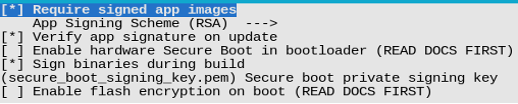
\includegraphics[width=0.7\textwidth]{D13Z/13-12}
    \caption{Enabling software secure boot for ESP32-C3}
\end{figure}

When software secure boot is enabled, during firmware building, the generated app firmware (referred to as origin\_app below) contains a public key, which will be used to verify the legitimacy of the new firmware \verb|new_app| sent via OTA upgrade. As shown in Figure 13.13, during OTA upgrades, after receiving the firmware and calling \verb|esp_ota_end()| or \verb|esp_ota_set_boot_partition()|, software secure boot will automatically use the public key in \verb|origin_app| to verify the digital signature attached to \verb|new_app|.

\begin{figure}[!h]
    \centering
    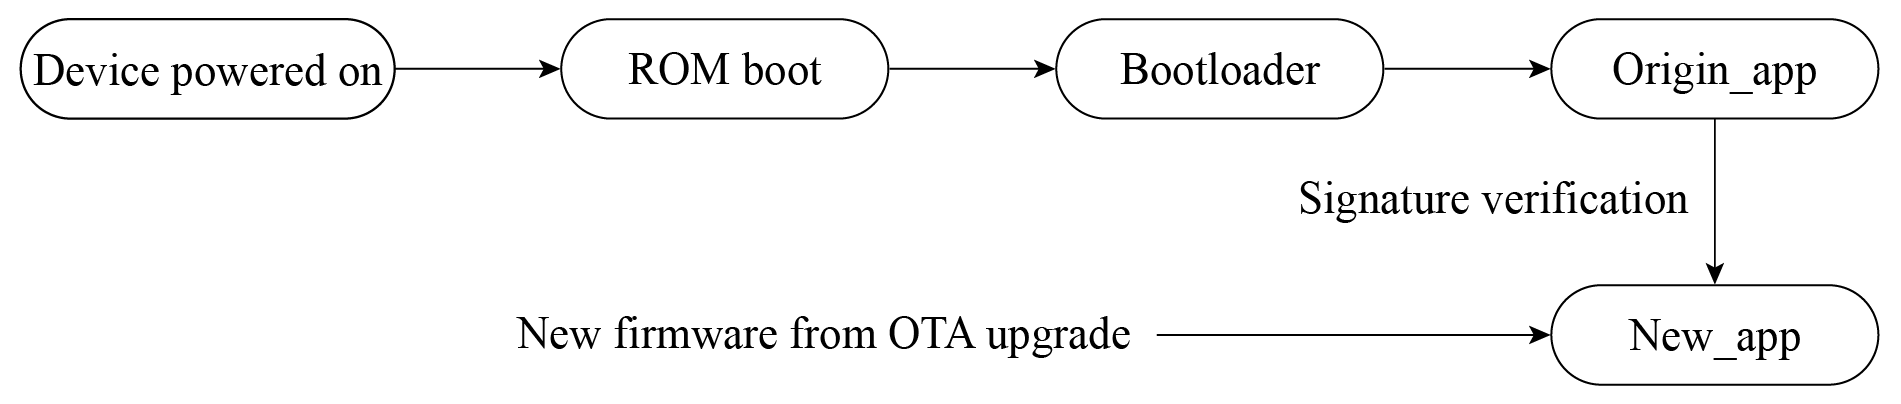
\includegraphics[width=0.8\textwidth]{D13Z/13-13}
    \caption{Software secure boot verifies new app firmware sent via OTA upgrades}
\end{figure}

When software secure boot is enabled, the app firmware sent to the device through OTA upgrade must be signed with a private key. There are two ways to achieve this:

\begin{enumerate}[label=(\arabic*)]
    \item As shown in Figure 13.12, configure the option \verb|Sign binaries during build|, and specify the directory of the private key file, then the app firmware can be automatically signed when compiling.
    \item Run the following command to sign the app firmware:
\end{enumerate}

\begin{codebloc}
\begin{tabular}{d}
\$ \textbf{espsecure.py sign\_data --version 2 --keyfile PRIVATE\_SIGNING\_KEY BINARY\_FILE}
\end{tabular}
\end{codebloc}

The above command directly modifies the current file and adds verification information to it. Use the \verb|--output| option to name the file after the signature is added. Using a command to sign firmware allows the signed private key to be stored on a remote server, rather than on the build machine, therefore, it is more convenient for batch signing on mass-produced devices.

Enabling software secure boot involves appending a signature block to the app firmware. This signature block encompasses the necessary data for signature verification. In the case of ESP32-C3, when utilising software secure boot, only the initial signature block holds validity. Conversely, when opting for hardware secure boot, up to three signature blocks are permitted, each capable of being signed with a distinct private key. Verification is considered successful as long as at least one of the signatures is valid. The data format of the signed app firmware of ESP32-C3 is shown in Figure 13.14.

\begin{figure}[!h]
    \centering
    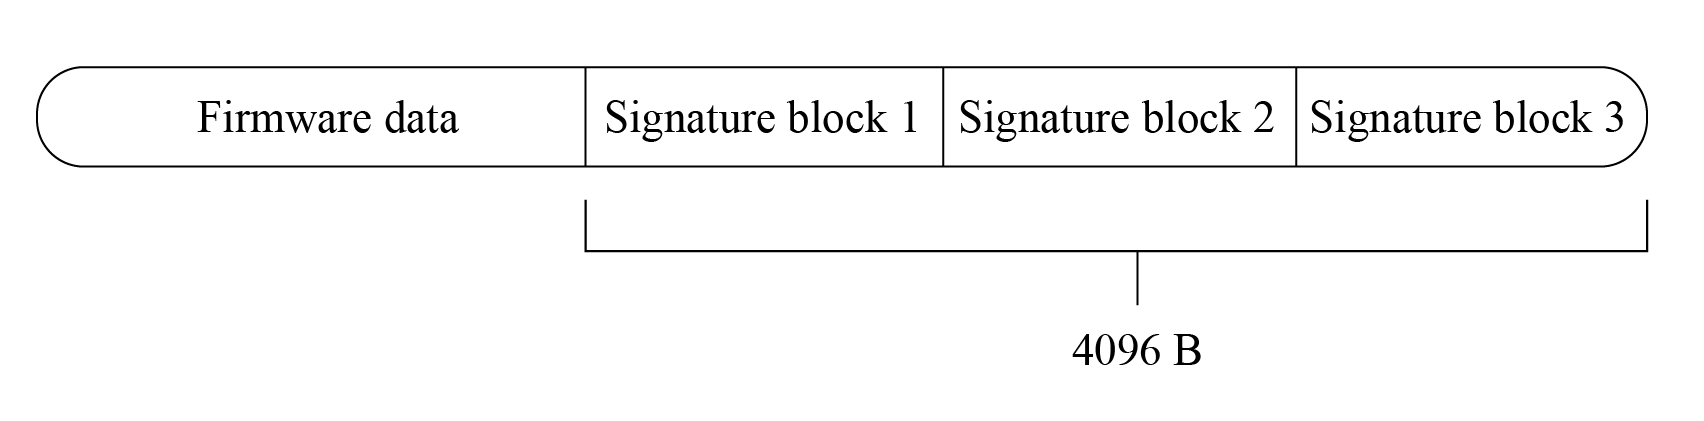
\includegraphics[width=0.9\textwidth]{D13Z/13-14}
    \caption{Data format of signed app firmware of ESP32-C3}
\end{figure}

In the software secure boot scheme, the public key used to verify the signature is compiled within the currently running app firmware and is automatically managed by the device. Users are not required to manage it manually. To obtain the content of the public key, use the following command to manually export the public key derived from the private key:

\begin{codebloc}
\begin{tabular}{d}
\$ \textbf{espsecure.py extract\_public\_key --version 2 --keyfile secure\_boot\_signing\_key.\newline pem pub\_key.pem}
\end{tabular}
\end{codebloc}

In this command, \verb|secure_boot_signing_key.pem| is the private key, and \verb|pub_key.pem| is the public key derived from the private key.

From the implementation principles of software secure boot, we can conclude that the scheme verifies the \verb|new_app| sent via OTA upgrade using the \verb|origin_app|. However, attackers have the potential to flash unauthorised bootloader and \verb|origin_app| onto the device through physical flashing, which cannot be managed by the software secure boot. As a result, software secure boot is more suitable for scenarios where the device is not susceptible to physical attacks. In the subsequent sections, we will delve into how the hardware secure boot scheme addresses physical attacks.

\subsection{Introduction to Hardware Secure Boot}
Hardware secure boot involves verification that is done via hardware.

It uses the data stored in eFuse to verify the legitimacy of firmware data. Relevant eFuses are shown in Table 13.3.

\begin{table}[h!]
    \renewcommand{\arraystretch}{1.4}
    \caption{eFuses used in verifying legitimacy of firmware data}
    \begin{tabular}{|>{\Centering}m{9em}|m{23.5em}|>{\Centering}m{6em}|}
        \hline
        \rowcolor{LightBlue} \textbf{eFuses}&\multicolumn{1}{c|}{\textbf{Description}}&\textbf{Length (bit)}\\
        \hline
        \verb|SECURE_BOOT_EN|&If set, hardware secure boot is enabled permanently.&1\\
        \hline
        \texttt{KEY\_PURPOSE\_\textit{X}}&\textit{X} is a natural number. For example, \verb|KEY_PURPOSE_1| is used to set the purpose of \verb|BLOCK_KEY1|.&4\\
        \hline
        \verb|BLOCK_KEYX|&If the corresponding \texttt{KEY\_PURPOSE\_\textit{X}} is set to \verb|SECURE_BOOT_DIGEST1|, then \verb|BLOCK_KEYX| will have the SHA256 digest of the public key.&256\\
        \hline
    \end{tabular}
\end{table}

Hardware secure boot supports not only all the functions of software secure boot described in Section 13.4.3, but also additional verifications on the bootloader and \verb|origin_app| firmware. Hardware secure boot scheme uses the same method of generating private-public key pair, and the same method of signing app firmware, as presented in Section 13.4.3.

When hardware secure boot is enabled, in addition to the app firmware, the bootloader also requires signing, using the same method and format as app firmware. In the event that the bootloader needs to be rebuilt and resigned, it is necessary to execute the command \verb|idf.py bootloader| separately. Additionally, the command \verb|idf.py -p PORT boot|\\ \verb|loader-flash| is required to flash the signed bootloader. Running \verb|idf.py flash| will only flash the signed app firmware and partition table, excluding the bootloader.

Hardware secure boot can be enabled as follows: 

\begin{enumerate}[label=(\arabic*)]
    \item Open the Project Configuration Menu, navigate to \verb|menuconfig → Security fea|\\ \verb|tures| and select the \verb|Enable hardware Secure Boot| option.
    \item If the firmware needs to be signed while compiling, specify the private key of the signature. As shown in Figure 13.15, specify the private key file through \verb|menuconfig → |\\ \verb|Security features → Secure Boot private key|. If the private key has not been generated, refer to Section 13.4.3 to export the private key. In addition, refer to Section 13.4.3 to sign the firmware using \verb|espsecure.py|.
    \item Run the command \verb|idf.py bootloader| to build the bootloader, and then \verb|idf.py |\\ \verb|-p PORT bootloader-flash| to flash the bootloader.
    \item Run \verb|idf.py flash monitor| to flash the app firmware and partition table.
    \item After the device is powered on, it will execute the just-built bootloader, which automatically sets the \verb|SECURE_BOOT_EN| flag in the eFuse, enabling permanent usage of hardware secure boot. Furthermore, the public key digest, which is attached to the signature block of the bootloader, will be written into \verb|BLOCK_KEY|. Figure 13.15 shows how to enable hardware secure boot during the compilation stage.
\end{enumerate}

\begin{figure}[!h]
    \centering
    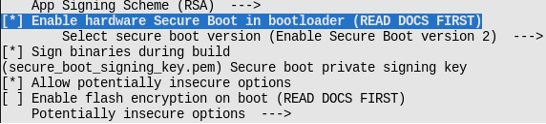
\includegraphics[width=0.7\textwidth]{D13Z/13-15}
    \caption{Enabling hardware secure boot during compilation}
\end{figure}

\note{
\vspace{2pt}
\begin{enumerate}[label=\arabic*.]
    \item When hardware secure boot is enabled, make sure to save the signed private key file, otherwise the updated bootloader and app firmware may not be sent to the device.
    \item Enabling secure boot will increase the size of bootloader, which might require updating partition table offset or reducing bootloader size. Refer to Section 13.3.4 for detailed instructions.
    \item If more content is added to the bootloader firmware, make sure the bootloader size does not exceed 0x10000.
    \item Hardware secure boot saves the SHA256 digest of the public key in eFuse, not the public key itself. This is because the public key itself contains a lot of data, but the eFuse space is limited.
\end{enumerate}
Visit \url{https://bookc3.espressif.com/bootloader} for more information about bootloader.
}

When hardware secure boot is enabled, the device will perform the following verification on updated bootloader and app firmware.

\begin{enumerate}[label=(\arabic*)]
    \item \textbf{Public key verification}. Upon device startup, ROM Boot will check the eFuse. If hardware secure boot is enabled, ROM checks the digest of the public key in the bootloader and validates if it matches the digest of the public key in eFuse. If they do not match, it means that the public key has been tampered with or damaged, and the boot is terminated; otherwise, the public key in the bootloader is considered correct, and the boot process continues.
    \item \textbf{Bootloader signature verification}. ROM Boot uses the public key to verify the bootloader signature. If the verification fails, the boot will be terminated; otherwise, the process continues.
    \item \textbf{\texttt{origin\_app} signature verification}. The bootloader uses the public key to verify the signature of \verb|origin_app|. If the verification fails, the boot process is terminated.
    \item \textbf{\texttt{new\_app} signature verification during OTA upgrades}. This is done through \verb|origin|\\ \verb|_app|, in a similar manner to software secure boot.
\end{enumerate}

Figure 13.16 shows the basic flow of signature verification done by hardware secure boot.

\begin{figure}[!h]
    \centering
    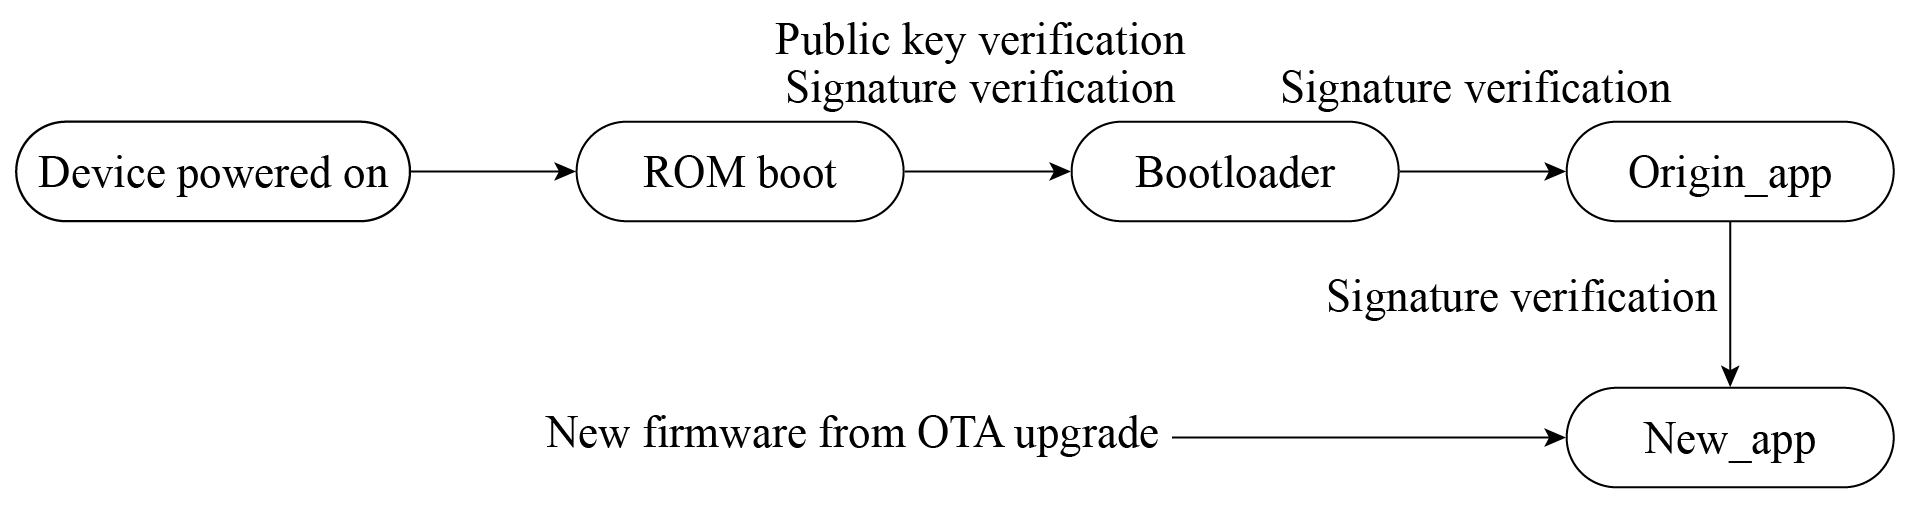
\includegraphics[width=0.8\textwidth]{D13Z/13-16}
    \caption{Basic flow of signature verification by hardware secure boot}
\end{figure}

\note{The complete signature verification process not only verifies signatures, but also verifies other data, such as the digest of the firmware.}

Hardware secure boot starts signature verification from ROM Boot, and then progresses to the bootloader, the \verb|origin_app| firmware, and finally the \verb|new_app| firmware, step by step, establishing a complete trust chain of \verb|ROM boot → bootloader → origin_app → |\\ \verb|new_app|. From the above-described process, it is not difficult to tell the differences between software secure boot and hardware secure boot, as outlined in Table 13.4.

\begin{table}[h!]
    \renewcommand{\arraystretch}{1.4}
    \caption{Differences between software secure boot and hardware secure boot}
    \begin{tabular}{|>{\Centering}m{10em}|>{\RaggedRight}m{13em}|>{\RaggedRight}m{15em}|}
        \hline
        \rowcolor{LightBlue} \textbf{Items}&\multicolumn{1}{c|}{\textbf{Software Secure Boot}}&\multicolumn{1}{c|}{\textbf{Hardware Secure Boot}}\\
        \hline
        Using eFuse?&\multicolumn{1}{c|}{No.}&\multicolumn{1}{c|}{Yes.}\\
        \hline
        Scope of established trust chain&\verb|origin_app → new_app|&A complete trust chain of \verb|ROM boot → bootloader →|\newline \verb|origin_app → new_app|\\
        \hline
        Can private key-public key pairs be replaced?&Yes. Re-flashing app firmware will enable a new private key-public key pair.&No. The public key digest is fixed in eFuse.\\
        \hline
        Can be disabled?&Yes. It can be disabled by re-flashing app.bin that does not have software secure boot enabled.&No. Once hardware secure boot is enabled, the SECURE\_BOOT\_EN in eFuse is burnt, which means it cannot be disabled.\\
        \hline
    \end{tabular}
\end{table}

The hardware secure boot scheme performs more verification during the process from ROM Boot to \verb|origin_app| execution, thus increasing the device startup time and the bootloader size. In the application scenarios where devices need to start up quickly, or small-sized bootloader is required, software secure boot is more suitable.

When hardware secure boot is enabled, there will be some restrictions applied to the device, including: 

\begin{itemize}[leftmargin=1.5em]
    \item The device can only run signed bootloader and app firmware. As a result, re-flashed bootloader and app firmware, or updated app firmware via OTA upgrades need to be signed with the corresponding private keys.
    \item In order to strengthen system security, by default, when hardware secure boot is enabled, JTAG debugging is disabled. Moreover, read protection of eFuse is disabled, and the unused signature slot in the eFuse is canceled. At the development stage, these functions can be retained through \verb|menuconfig → Security features → Potentially |\\ \verb|insecure options|. At mass production stage, these functions should be disabled by default to enhance the overall security of the device.
    \item When hardware secure boot is enabled, the device’s UART download function will change, depending on the selected option of \verb|menuconfig → security features → UART|\\ \verb|ROM download mode|. There are three options of \verb|UART ROM download mode|, as shown in Table 13.5.
\end{itemize}

\begin{table}[h!]
    \renewcommand{\arraystretch}{1.4}
    \caption{Options of \texttt{UART ROM download mode}}
    \begin{tabular}{|>{\Centering}m{13em}|>{\RaggedRight}m{25.5em}|}
        \hline
        \rowcolor{LightBlue} \textbf{Option}&\multicolumn{1}{c|}{\textbf{Description}}\\
        \hline
        \verb|Enabled|&Retains flash read/write through serial port\\
        \hline
        \verb|Switch to Secure mode|&Retains only basic functions of flash read/write through serial port. Advanced functions (such as downloading encrypted firmware) are forbidden.\\
        \hline
        \verb|Permanently disabled|&Disables flash read/write through serial port\\
        \hline
    \end{tabular}
\end{table}

So far, we have learnt the basic principles and common usage of hardware secure boot. There are also advanced usages of the scheme, such as using multiple signatures or cancelling invalid public keys.

\note{Visit \url{https://bookc3.espressif.com/secure-boot-v2} for user guides on Secure Boot v2.}

\subsection{Examples}
The secure boot solution features have been seamlessly integrated into ESP-IDF. By familiarising yourself with the implementation principles and configuring the appropriate options in the \verb|menuconfig|, you can easily enable these features according to your requirements. In comparison to the software secure boot solution, the hardware secure boot provides a more comprehensive verification of firmware validity. Thus, it is recommended to utilise the hardware secure boot solution to enhance device security during the mass production stage. This section will present several examples of enabling hardware secure boot, which can be utilised for testing purposes. Furthermore, if you encounter any errors while sending new firmware to the device using hardware secure boot, the following log messages can serve as a reference for troubleshooting.

When hardware secure boot is enabled according to the steps described in 13.4.4, starting up the device for the first time will get the following log message:

\begin{codebloc}
\begin{tabular}{d}
\vspace{2pt}
\begin{verbatim}
I (10251) secure_boot_v2: Secure boot V2 is not enabled yet and eFsue digest 
keys are not set
I (10256) secure_boot_v2: Verifying with RSA-PSS...
I (10254) secure_boot_v2: Signature verified successfully!
I (10272) boot: boot: Loaded app from partition at offset 0X120000
\end{verbatim}
\verb|I (10274) secure_boot_v2: Enabling secure boot V2...|
\end{tabular}
\end{codebloc}

Re-powering up the device will get the following message:

\begin{codebloc}
\begin{tabular}{d}
\vspace{2pt}
\begin{verbatim}
ESP-ROM:esp32c3-api1-20210207
Build:Feb 7 2021
rst:0x1 (POWERON),boot:0xC(SPI_FAST_FLASH_BOOT)
SPIWP:0xee
mode:DIO, clock div:1
Valid Secure Boot key blocks: 0
Secure Boot verification succeeded
load:0x3fcd6268,len:0x2ebc
load:0x403ce000,len:0x928
load:0x403d0000,len:0x4ce4
entry 0x403ce000
\end{verbatim}
\verb|I (71) boot: ESP-IDF v4.3.2-2741-g7c0fa3fc70 2nd stage bootloader|
\end{tabular}
\end{codebloc}

Flashing unsigned bootloader to the device will get the following error message and terminate boot process.

\begin{codebloc}
\begin{tabular}{d}
\vspace{2pt}
\begin{verbatim}
ESP-ROM:esp32c3-api1-20210207
Build:Feb 7 2021
rst:0x1 (POWERON),boot:0xC(SPI_FAST_FLASH_BOOT)
SPIWP:0xee
mode:DIO, clock div:1
Valid secure boot key blocks: 0
No signature block magic byte found at signature sector (found 0xcd not 0xe7). 
Image not V2 signed?
secure boot verification failed
\end{verbatim}
\verb|ets_main.c 333|
\end{tabular}
\end{codebloc}

Flashing unsigned app firmware to the device will get the following error message and terminate boot process.

\begin{codebloc}
\begin{tabular}{d}
\verb|I (310) esp_image: Verifying image signature...|
\end{tabular}
\end{codebloc}

\begin{codebloc}
\begin{tabular}{d}
\vspace{2pt}
\begin{verbatim}
I (312) secure_boot_v2: Verifying with RSA-PSS...
No signature block magic byte found at signature sector (found 0x41 not 0xe7). 
Image not V2 signed?
E (326) secure_boot_v2: Secure Boot V2 verification failed.
E (332) esp_image: Secure boot signature verification failed
I (339) esp_image: Calculating simple hash to check for corruption...
\end{verbatim}
\verb|W (418) esp_image: image valid, signature bad|
\end{tabular}
\end{codebloc}

Sending unsigned app firmware to the device through OTA upgrade will cause signature verification failure, thus ending the data transmission, and preventing firmware loading.

\begin{codebloc}
\begin{tabular}{d}
\fontsize{9pt}{10pt}\selectfont
\vspace{2pt}
\begin{verbatim}
I (4487) simple_ota_example: Starting OTA example
I (5657) esp_https_ota: Starting OTA...
I (5657) esp_https_ota: Writing to partition subtype 16 at offset 0x120000
I (26557) esp_image: segment 0: paddr=00120020 vaddr=3c0a0020 size=1b488h (111752) map
I (26567) esp_image: segment 1: paddr=0013b4b0 vaddr=3fc8d800 size=02b10h ( 11024) 
I (26567) esp_image: segment 2: paddr=0013dfc8 vaddr=40380000 size=02050h (  8272) 
I (26577) esp_image: segment 3: paddr=00140020 vaddr=42000020 size=9d9ech (645612) map
I (26667) esp_image: segment 4: paddr=001dda14 vaddr=40382050 size=0b60ch ( 46604) 
I (26667) esp_image: segment 5: paddr=001e9028 vaddr=50000000 size=00010h (    16) 
I (26667) esp_image: Verifying image signature...
I (26677) secure_boot_v2: Take trusted digest key(s) from eFuse block(s)
E (26687) esp_image: Secure boot signature verification failed
I (26687) esp_image: Calculating simple hash to check for corruption...
W (26757) esp_image: image valid, signature bad
\end{verbatim}
\verb|E (26767) simple_ota_example: Firmware upgrade failed|
\end{tabular}
\end{codebloc}

\section{Practice: Security Features In Mass Production}
\subsection{Flash Encryption and Secure Boot}
The flash encryption scheme is primarily used to safeguard the confidentiality of data stored on the device’s flash, while the secure boot scheme is focused on ensuring the legitimacy of firmware data. For optimal device security, it is recommended to utilise both schemes in conjunction. As shown in Figure 13.17, flash encryption and secure boot can be simultaneously enabled during the firmware building process.

\begin{figure}[!h]
    \centering
    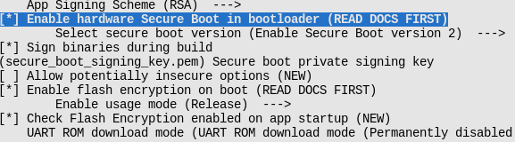
\includegraphics[width=0.7\textwidth]{D13Z/13-17}
    \caption{Enabling flash encryption and secure boot through menuconfig}
\end{figure}

Additionally, when using flash encryption and secure boot, pay attention to the following to enhance device security:

\begin{itemize}[leftmargin=1.5em]
    \item Generate different flash encryption keys for different devices.
    \item Switch \verb|UART ROM download mode| to \verb|Secure mode| or \verb|disabled mode| through \verb|menuconfig → Security features|.
    \item Secure the private key for signature in a private location so that it will not be lost or disclosed. Sign only on a secure device. If the key for flash encryption is exported, also save it in a private location.
\end{itemize}

\subsection{Enabling Flash Encryption and Secure Boot with Batch Flash Tools}
For Linux systems, tools such as \verb|esptool.py| and \verb|espsecure.py| can be used to configure security features or flash firmware data. These tools help leverage security features with more flexibility.

For Windows systems, the flash download tool (from \url{https://www.espressif.com/zh-hans/support/download/other-tools}) can flash firmware in batch, with both secure boot and flash encryption enabled simultaneously. Open the \verb|configure/esp32c3/security| file in the tool’s directory, and configure the settings of secure boot and flash encryption. The security configuration file is shown in Figure 13.18.

\begin{figure}[!h]
    \centering
    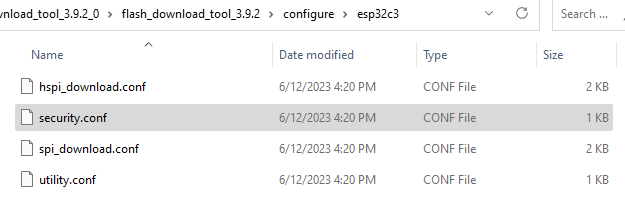
\includegraphics[width=0.6\textwidth,frame]{D13Z/13-18}
    \caption{Security configuration file in flash download tool}
\end{figure}

\note{If the \texttt{security} file does not show when the directory is opened for the first time, quit the program first and re-open it, then the file will show.}

The default security configurations in the \verb|security| file are as follows:

\begin{codebloc}
\begin{tabular}{d}
\vspace{2pt}
\begin{verbatim}
1.	 [SECURE BOOT]
2.  secure_boot_en = False      //Enable secure boot?
3.	
4.	 [FLASH ENCRYPTION]
5.  flash_encryption_en = False //Enable flash encryption?
6.  reserved_burn_times = 0     //Reserve flash encryption in development mode?
7.          //The number of times control bit SPI_BOOT_CRYPT_CNT can be burnt
8.	
9.	 [ENCRYPTION KEYS SAVE]
\end{verbatim}
\verb|10. keys_save_enable = False    //Save the key for flash encryption locally?|
\end{tabular}
\end{codebloc}

\begin{codebloc}
\begin{tabular}{d}
\vspace{2pt}
\begin{verbatim}
11. encrypt_keys_enable = False //Encrypt the key saved locally?
12. encrypt_keys_aeskey_path =  //Key path
13.	
14.  [DISABLE FUNC]
15. jtag_disable = False
16. dl_encrypt_disable = False
17. dl_decrypt_disable = False
\end{verbatim}
\verb|18. dl_cache_disable = False|
\end{tabular}
\end{codebloc}

Please refer to the user manual of the flash download tool for more information.

\note{At production stage when both flash encryption and secure boot are enabled on the device, it is important to use a standard and stable \textbf{power supply}, otherwise the device may be damaged permanently.}

\subsection{Enabling Flash Encryption and Secure Boot in Smart Light Project}
Different from other solutions presented in this book, flash encryption and secure boot can be used almost “out of the box”, without the need for additional coding. These security schemes can be conveniently enabled by configuring the \verb|menuconfig| settings. For a smart lighting system, we recommend using flash encryption, NVS encryption, and hardware secure boot simultaneously to enhance the overall device security to its maximum potential.

\section{Summary}
This chapter first introduces two key aspects of IoT device security: data storage and data transmission. These aspects have specific requirements for data integrity, confidentiality, and legitimacy. Then, the chapter proceeds to discuss several solutions that address these security concerns, including:

\begin{itemize}[leftmargin=1.5em]
    \item \textbf{Data integrity verification algorithm} verifies the integrity of firmware data during the firmware loading process or OTA upgrades. 
    \item \textbf{Flash encryption} and \textbf{NVS encryption} safeguard the confidentiality of data stored in flash memory and prevent unauthorised access to key data. Encrypted data can only be loaded after decryption using a specific key. Enabling flash encryption ensures that even if the data is obtained from the flash, it cannot be copied to another device for loading, thereby protecting the intellectual property rights of software developers. 
    \item \textbf{Secure boot scheme} verifies the authenticity and legitimacy of firmware data, ensuring that only firmware from authenticated sources is allowed to run on the device.
\end{itemize}

Finally, the chapter provides a brief overview of how to enable flash encryption and secure boot using the mass production download tools.

\end{document}